\documentclass[10pt,conference,compsocconf]{IEEEtran}

\usepackage{hyperref}
\usepackage{graphicx}
\usepackage{amsmath}
\usepackage{booktabs}
\usepackage{amssymb}

\graphicspath{{../outputs/plots/}{../outputs/figures/}}

\begin{document}

\title{Asynchronous SGD: Delay, Momentum, and Generalization}

\author{
  Alexandre Potocnik \quad Aleksandar Mihaylov \quad Ilia Badanin \\
  \textit{EPFL, Switzerland --- CS-439 Optimization for ML}
}

\maketitle

\begin{abstract}
Gradient staleness from asynchronous training degrades convergence and
interacts non-trivially with momentum.
We investigate three questions: (1)~how delay affects convergence speed
and final accuracy; (2)~how momentum interacts with delay and whether
theory-guided scheduling recovers performance; and (3)~whether gradient
staleness acts as a regularizer analogous to dropout.
For question~1, delay degrades accuracy monotonically ($-29.5$\,pp under
$\beta{=}0$ from $\tau{=}0$ to $\tau{=}20$), with harm concentrated at
LR-decay transitions; at $\mathrm{E}[\tau]{=}64$, LR scaling
$\eta \to \eta/\tau$ recovers 64.5\% under geometric delay vs.\ 31.3\%
under FIFO ($+33.2$\,pp, $\beta{=}0.9$).
For question~2, $\beta{=}0.9$ collapses catastrophically under deterministic
delay (90.3\% to below 11\% at $\tau{=}20$), consistent with Liu et
al.~\cite{liu2018momentum}; an adaptive schedule tracking the bound recovers
up to $+5.9$\,pp, and the delay distribution matters as much as its magnitude.
For question~3, weight decay and gradient staleness act on independent axes:
varying $\tau$ leaves the weight-norm trajectory unchanged while $\lambda$
precisely controls it, so weight decay transfers directly to delayed settings.
\end{abstract}

% =========================================================================
\section{Introduction}
% =========================================================================

% Stochastic gradient descent is the workhorse of deep learning, but
% wall-clock training time on a single processor is a bottleneck at scale.
% Asynchronous SGD~\cite{recht2011hogwild} sidesteps synchronization overhead
% by allowing workers to apply gradients without waiting for each other,
% producing \emph{stale} gradients: a gradient computed on $\theta_t$ is
% applied at time $t{+}\tau$ when the model has already advanced to
% $\theta_{t+\tau}$.
% The practical impact of this staleness on accuracy and convergence depends
% critically on both the magnitude and the \emph{distribution} of the delay.
% Studying this empirically in a real distributed system introduces
% confounders (hardware variance, network jitter, synchronization overhead)
% that make it difficult to isolate the effect of staleness itself.
% We therefore adopt a \emph{controlled simulation} approach: a single
% sequential process injects gradients from a buffer, precisely controlling
% the staleness at each step.
% This allows clean isolation of delay effects but does not capture
% system-level phenomena such as worker heterogeneity or communication overlap.

% Three concrete questions motivate this project.
% First, does delay degrade accuracy monotonically, and does it slow
% convergence uniformly across training phases?
% Second, how does explicit momentum interact with staleness, does the
% distribution of delays (deterministic vs.\ stochastic) change this
% interaction, and can theoretical guarantees guide adaptive schedule design?
% Third, can gradient noise from staleness act as a regularizer analogous
% to dropout, improving generalization?

% Our contributions for question~1 are:
% \begin{itemize}
%   \item Learning curves across $\tau \in \{0,2,5,10,20\}$ showing that delay
%         shifts convergence trajectories downward and rightward, with
%         disproportionate harm at LR-decay milestones: at $\tau{=}20$ the
%         model effectively stalls after epoch~30 because stale gradients
%         cannot track the post-decay landscape.
%   \item A convergence-speed analysis showing that the 80\% accuracy threshold
%         is reached at epoch~26 for $\tau{=}0$ but is never reached at
%         $\tau{=}20$; the 85\% threshold is unattainable beyond $\tau{=}5$.
%   \item Evidence that delay does not reduce the train-test gap, ruling out
%         an implicit-regularisation interpretation: staleness uniformly
%         degrades optimisation without changing the overfitting regime.
% \end{itemize}

% % [Q3 TEAMMATE Aleksandar: expand on question 3 and your contributions here]

% Our contributions for question~2 are:
% \begin{itemize}
%   \item A $\tau \times \beta$ grid (45 runs) showing that $\beta{=}0.9$
%         is catastrophically unstable at any nonzero \emph{deterministic}
%         delay, consistent with the Liu et al.\ bound
%         $\tau \lesssim (1-\mu)^2/\eta$.
%   \item A matched geometric-delay sweep ($\tau_t \sim \mathrm{Geom}(1/M)$,
%         45 runs) revealing that the delay distribution type fundamentally
%         changes the momentum-delay interaction: at the same average staleness,
%         stochastic delay is safer for $\beta{=}0$ but more dangerous for
%         $\beta{=}0.9$.
%   \item A negative result for the Mitliagkas equivalence
%         conjecture~\cite{mitliagkas2014async} even under geometric delay,
%         confirming it does not hold empirically on ResNet-20/CIFAR-10.
%   \item Negative explicit momentum ($\beta \in [-0.9, 0]$) as a
%         theoretically grounded compensation, yielding a $+13.3$\,pp gain
%         at $\tau{=}20$.
%   \item An adaptive momentum schedule tracking
%         $\mu_\mathrm{safe}(\eta_t) = 1 - \sqrt{\tau \eta_t}$ as the LR
%         decays, consistently outperforming all fixed-$\beta$ baselines under
%         both delay regimes.
% \end{itemize}

Recht et al.~\cite{recht2011hogwild} introduced Hogwild!, a lock-free asynchronous SGD
algorithm in which multiple workers read and write shared model parameters without
synchronization. Despite the resulting gradient staleness, they showed that under
sparsity assumptions, convergence is preserved with nearly the same sample efficiency
as sequential SGD. This result established asynchronous SGD as a practical approach to
speeding up training with minimal accuracy loss.

Running true asynchronous training on CPU is impractical at scale, so we simulate it
sequentially by injecting controlled gradient staleness via a buffer. We use two delay
models: a deterministic FIFO queue with fixed delay $\tau$ and a stochastic geometric
model, $\tau_t \sim \mathrm{Geom}(1/M) - 1$, following Mitliagkas et al.~\cite{mitliagkas2014async}.
The geometric model matches the service-time distribution of $M$ parallel workers in an
M/M/1 queue and is therefore a principled proxy for real distributed systems.
Mitliagkas et al.\ further showed that such asynchronous updates introduce an
\emph{implicit momentum} term, connecting gradient staleness to explicit momentum methods.

We contributed (1) a systematic empirical analysis of delayed SGD across delay
magnitudes and distributions; (2) an adaptive momentum schedule grounded in
the Liu et al.\ bound~\cite{liu2018momentum} that consistently outperforms
fixed-$\beta$ baselines; and (3) an investigation of gradient staleness as a
potential implicit regularizer.

% =========================================================================
\section{Models and Methods}
\label{sec:methods}
% =========================================================================

\subsection{Common Setup}
\label{common_setup}

All experiments train ResNet-20~\cite{he2016resnet} on
CIFAR-10~\cite{krizhevsky2009cifar} (50k/10k split).
Base learning rate $\eta{=}0.1$, decayed by $\times 0.1$ at epochs 30 and
40 (50 total), batch size 128, weight decay $10^{-4}$. The source code for the ResNet-20 implementation was taken from Idelbayev~\cite{Idelbayev18a}. 
Every configuration is run with three random seeds \{42, 123, 456\}; we
report mean $\pm$ standard deviation of final test accuracy.

\subsection{Delay Simulation}

All delay experiments run in a \textbf{single sequential process}.
No workers, threads, or network communication are involved.
Staleness is injected artificially via a gradient buffer: at each step,
a fresh gradient is computed and stored, and a \emph{stale} gradient
from the buffer is applied to the parameters.
This design gives exact, reproducible control over the delay distribution
and eliminates confounders from real distributed systems, at the cost of
not modelling system-level effects.

\paragraph{$\tau$-Delayed Gradient Descent}
In standard gradient descent (GD), the parameter update at iteration
$t$ uses a gradient evaluated at the current iterate $\theta_t$. In the
delayed setting, the gradient applied at step $t$ was instead computed on
a \emph{past} iterate $\theta_{t-\tau_t}$, where $\tau_t \geq 0$ is the
staleness of that gradient. The update rule becomes
\begin{equation}
    \theta_{t+1} \;=\; \theta_t \;-\; \eta_t \, g\!\left(\theta_{t-\tau_t}\right),
    \label{eq:delayed-sgd}
\end{equation}
Setting $\tau_t \equiv 0$ recovers vanilla GD (see Appendix for notation).

\paragraph{Deterministic (FIFO) delay}
A FIFO buffer of depth $\tau$ is maintained.
After computing a fresh gradient on $\theta_t$, we push it onto the buffer
and apply the oldest buffered gradient to the parameters.
This gives a \emph{deterministic} staleness of exactly $\tau$ steps at
every update --- a controlled baseline that isolates delay magnitude.

\paragraph{Geometric (stochastic) delay}
To match the M/M/1 queue model from which Mitliagkas et
al.~\cite{mitliagkas2014async} derive their implicit-momentum result,
we sample a fresh delay at every step:
\begin{equation}
  \tau_t \sim \mathrm{Geom}(1/M) - 1, \qquad \mathrm{E}[\tau_t] = M-1.
\end{equation}
We choose $M \in \{1, 3, 6, 11, 21\}$ so that $\mathrm{E}[\tau] \in
\{0, 2, 5, 10, 20\}$ matches the deterministic grid exactly, enabling
direct comparison at the same average staleness.
A rolling buffer stores the last $5M$ gradient snapshots; each step
looks up the one sampled by $\tau_t$.

\paragraph{Optimizer}
All experiments use standard SGD with momentum.
For experiments requiring negative momentum, PyTorch's \texttt{SGD} rejects
$\beta < 0$, so we implement a custom \texttt{SGDMomentum} supporting any
$\beta \in \mathbb{R}$:
\begin{equation}
  v_t = \beta v_{t-1} + g_t,\qquad \theta_t = \theta_{t-1} - \eta v_t.
\end{equation}

\paragraph{Regularization experiments} 
For the experiments relating regularization to staleness, the changes described below alter the common setup (cf.~\ref{common_setup}). 
To isolate the interaction between staleness and explicit regularization,
we strip the optimizer of all confounding mechanisms. Momentum is set to
$\beta=0$ throughout, since momentum is known to interact strongly with
delay~\cite{mitliagkas2014async} and would obscure the effect of weight
decay. Weight decay is fixed at $\lambda=0$ unless it is the variable
under study. The learning rate is held constant at its initial value
$\eta=0.1$ with no decay schedule, to eliminate any possibility of the
schedule itself acting as an implicit regularizer and confounding our
measurements.

% =========================================================================
\section{Results}
\label{sec:results}
% =========================================================================

\subsection{Effect of Delay on Convergence}

\paragraph{Monotone accuracy degradation.}
Under $\beta{=}0$, final test accuracy drops monotonically from 87.2\% at
$\tau{=}0$ to 57.7\% at $\tau{=}20$, with the largest fall beyond $\tau{=}10$
where the model fails to reduce training loss.
The train--test gap \emph{narrows} with $\tau$ (Appendix, Fig.~\ref{fig:q1-gap}),
consistent with Deng et al.~\cite{deng2025generalizability}:
staleness harms optimisation, not generalisation.

\begin{figure}[tbp]
  \centering
  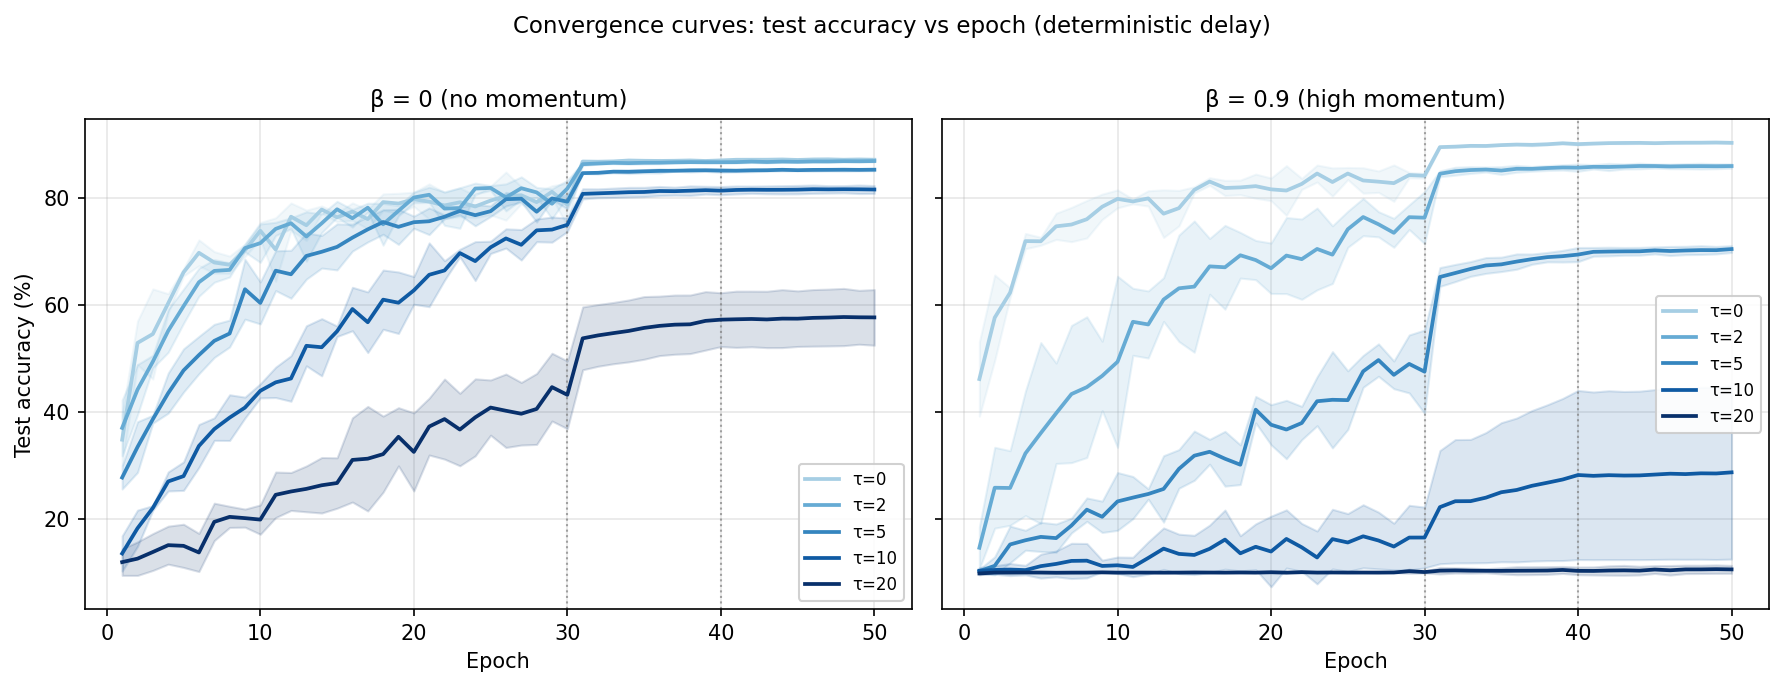
\includegraphics[width=\columnwidth]{plot_Q1_convergence_curves}
  \caption{Test accuracy vs.\ epoch for $\beta{=}0$ (left) and $\beta{=}0.9$
           (right) across $\tau \in \{0,2,5,10,20\}$ (deterministic delay).
           Mean over 3 seeds, shading $\pm$std.
           Dotted vertical lines mark LR decay milestones (epochs 30, 40).}
  \label{fig:q1-curves}
\end{figure}

\subsection{Momentum Collapse and Recovery}
\label{momentum_vs_delay}
Under delay, the benefit of momentum reverses sharply: at $\tau{=}20$,
$\beta{=}0.9$ collapses to 10.6\% (random-class level, Appendix
Fig.~\ref{fig:momentum-collapse}).
These results are consistent with the safe-momentum bound of Liu et
al.~\cite{liu2018momentum}, $\mu_\mathrm{safe} = 1 - \sqrt{\tau \cdot \eta}$:
at $\eta{=}0.1$, $\beta{=}0.9$ exceeds this bound for any $\tau \geq 1$.

\paragraph{Mitliagkas equivalence.}

Mitliagkas et al. \cite{mitliagkas2014async} conjecture that $M$ async workers with geometric
staleness induce implicit momentum $\mu_S{=}(M{-}1)/M$, making
$(M,\,\beta{=}0)$ equivalent to $(\tau{=}0,\,\beta{=}\mu_S)$.
We test this in its original regime (geometric delay): even there, the
equivalence does not hold --- at $M{=}6$, the geometric-delay run falls
$-4.5$\,pp short of the explicit-momentum baseline.
The conjecture does not generalise to deep learning with step-decay
schedules, consistent with Liu et al.'s refutation~\cite{liu2018momentum}.
\paragraph{Negative momentum (Exp~F).}
At $\tau{=}20$, the best fixed negative value ($\beta{=}{-}0.9$) reaches
71.0\%, a $+13.3$\,pp gain over the $\beta{=}0$ baseline of 57.7\%;
gains diminish at smaller delays (Appendix, Fig.~\ref{fig:neg-momentum}).

\paragraph{Adaptive schedule (Exp~G).}
We apply the Liu bound ($\mu_\mathrm{safe} = 1 - \sqrt{\tau \cdot \eta_t}$)
as an adaptive schedule, noting it was derived for a fixed-LR non-convex
setting rather than our step-decay regime.
Figure~\ref{fig:adaptive-summary} compares four schedules against fixed
baselines.
The \texttt{above\_bound} schedule ($\mu = \min(0.95,\,\mu_\mathrm{safe}+0.3)$)
achieves the best accuracy: 88.3\% at $\tau{=}5$, 85.1\% at $\tau{=}10$,
63.6\% at $\tau{=}20$ --- outperforming $\beta{=}0$ by up to $+5.9$\,pp.
That operating above the bound remains stable suggests it is conservative
outside its original regime.

\begin{figure}[tbp]
  \centering
  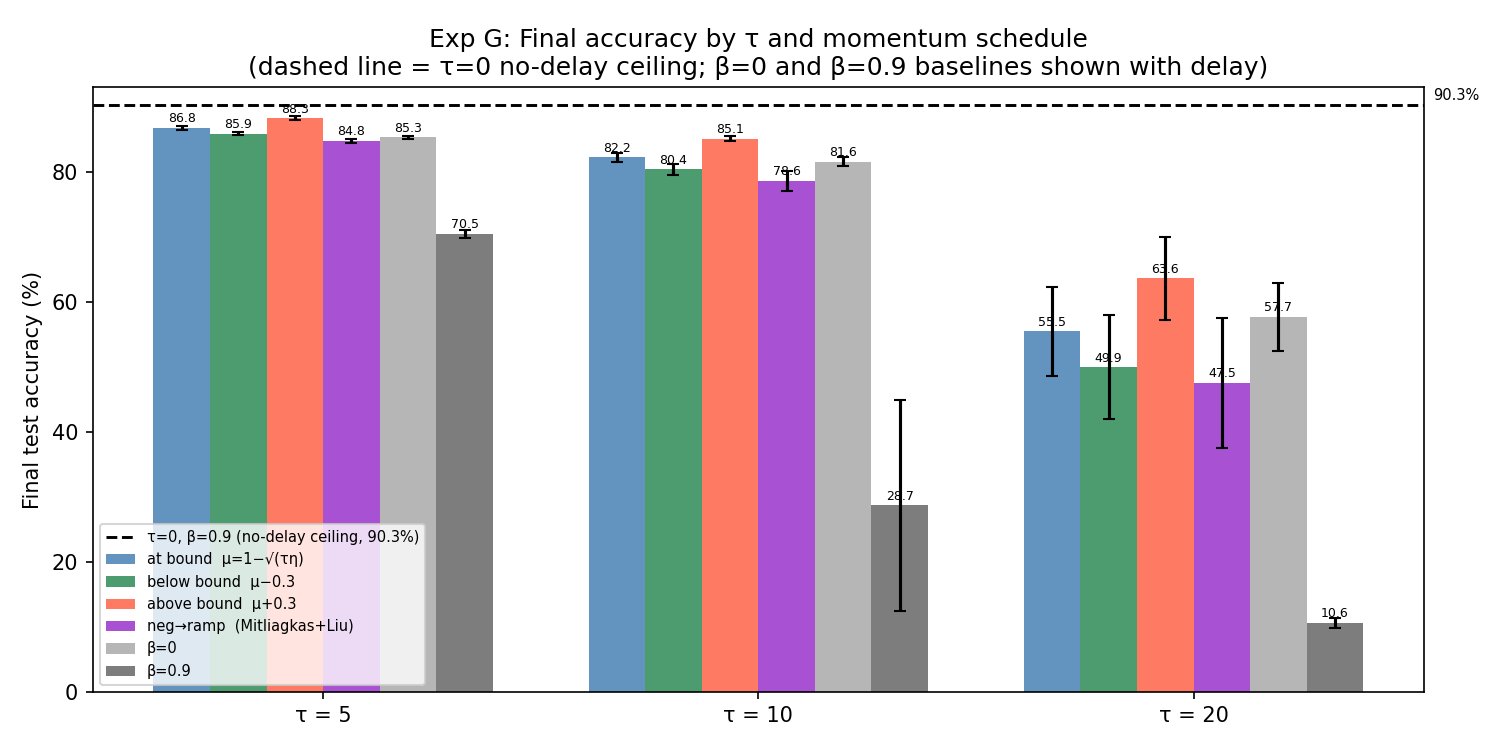
\includegraphics[width=\columnwidth]{plot_L2_adaptive_summary}
  \caption{Adaptive vs.\ fixed momentum under deterministic delay: final
           test accuracy by schedule and $\tau$.
           Dashed line marks the no-delay ceiling ($\tau{=}0$, $\beta{=}0.9$,
           90.3\%). \texttt{above\_bound} outperforms all fixed-$\beta$
           baselines at every delay.}
  \label{fig:adaptive-summary}
\end{figure}

\subsection{Delay Distribution Matters: Geometric vs.\ Deterministic}

\paragraph{$\beta{=}0$ (no momentum).}
Figure~\ref{fig:geo-comparison} shows geo is substantially more resilient
than det at matched staleness.
At $\mathrm{E}[\tau]{=}20$ (M=21), geo reaches 82.1\% vs.\ det 57.7\%
($+24.4$\,pp): roughly $1/M$ steps receive a fresh gradient under
geometric delay, periodically correcting the trajectory.

\paragraph{$\beta{=}0.9$ (high momentum).}
The roles reverse at medium-to-high staleness.
At $\mathrm{E}[\tau]{=}10$, geometric delay collapses completely
(9.9\%, random guessing) while deterministic delay degrades more
gracefully (28.7\%).
The geometric tail produces occasional extreme lags ($\tau_t \gg
\mathrm{E}[\tau]$) that corrupt the momentum accumulator; with $\beta{=}0.9$
the velocity is sticky and cannot recover.

\begin{figure}[tbp]
  \centering
  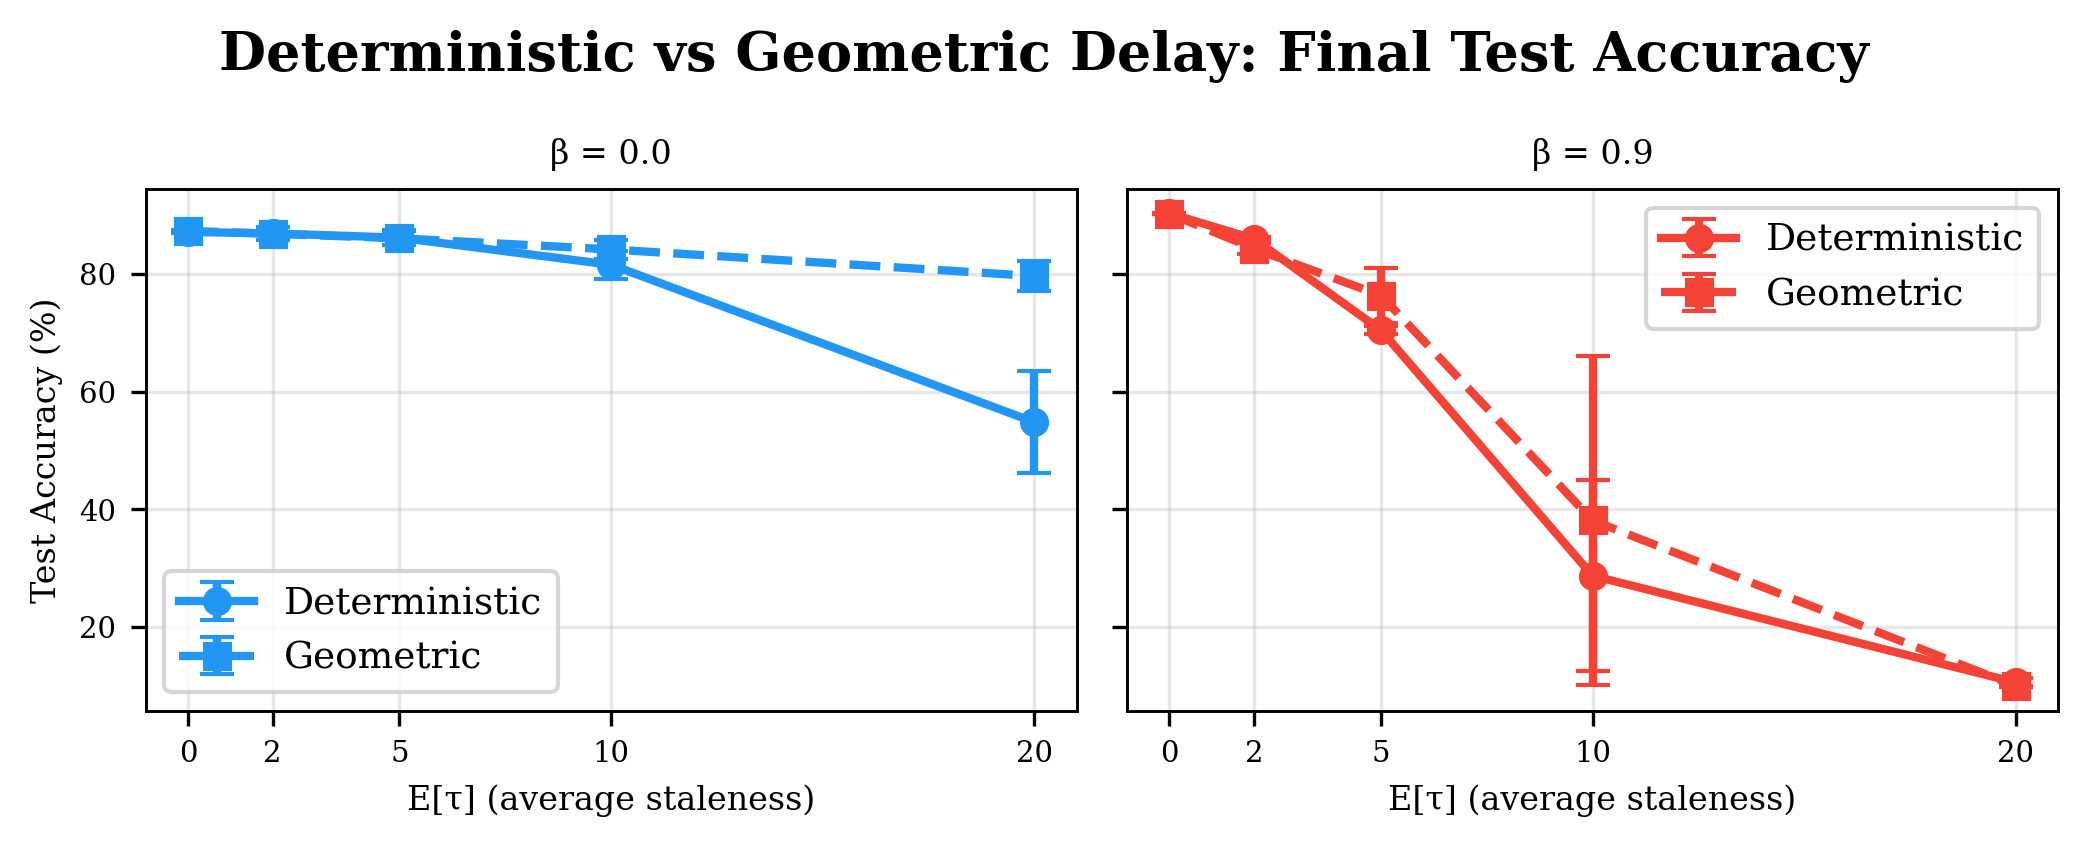
\includegraphics[width=\columnwidth]{plot_geo_step3_comparison}
  \caption{Final test accuracy vs.\ average staleness for deterministic
           (solid) and geometric (dashed) delay.
           For $\beta{=}0$, geometric delay is substantially more resilient.
           For $\beta{=}0.9$, geometric delay collapses faster due to
           momentum amplifying rare extreme-lag events.}
  \label{fig:geo-comparison}
\end{figure}



% =========================================================================
\subsection{LR Correction Rescues Convergence at High Staleness}
\label{sec:lrs-rescue}

Scaling $\eta \to \eta/\tau$ or $\eta \to \eta/\sqrt{\tau}$ compensates
for the gradient-variance inflation under large delays.
Figure~\ref{fig:lrs-rescue} shows the effect at $\tau{=}64$ (FIFO) and
$\mathrm{E}[\tau]{=}64$ (geometric, $M{=}65$) for both $\beta{=}0$ and $\beta{=}0.9$.
Without correction, $\beta{=}0.9$ collapses to ${\approx}10\%$ in both regimes.
For $\beta{=}0.9$, scaling $\eta \to \eta/\tau$ ($\mathrm{lrs}{=}1/64$) gives
the best recovery: FIFO reaches 31.3\% and geometric reaches \textbf{64.5\%}
($+33.2$\,pp gap).
For $\beta{=}0$, the optimal scale is only $\eta/\sqrt{\tau}$
($\mathrm{lrs}{=}1/\sqrt{64}{\approx}0.125$): pushing further to $\eta/\tau$ \emph{hurts}
performance, suggesting that the momentum accumulator drives the need for
aggressive LR reduction.

\begin{figure}[tbp]
  \centering
  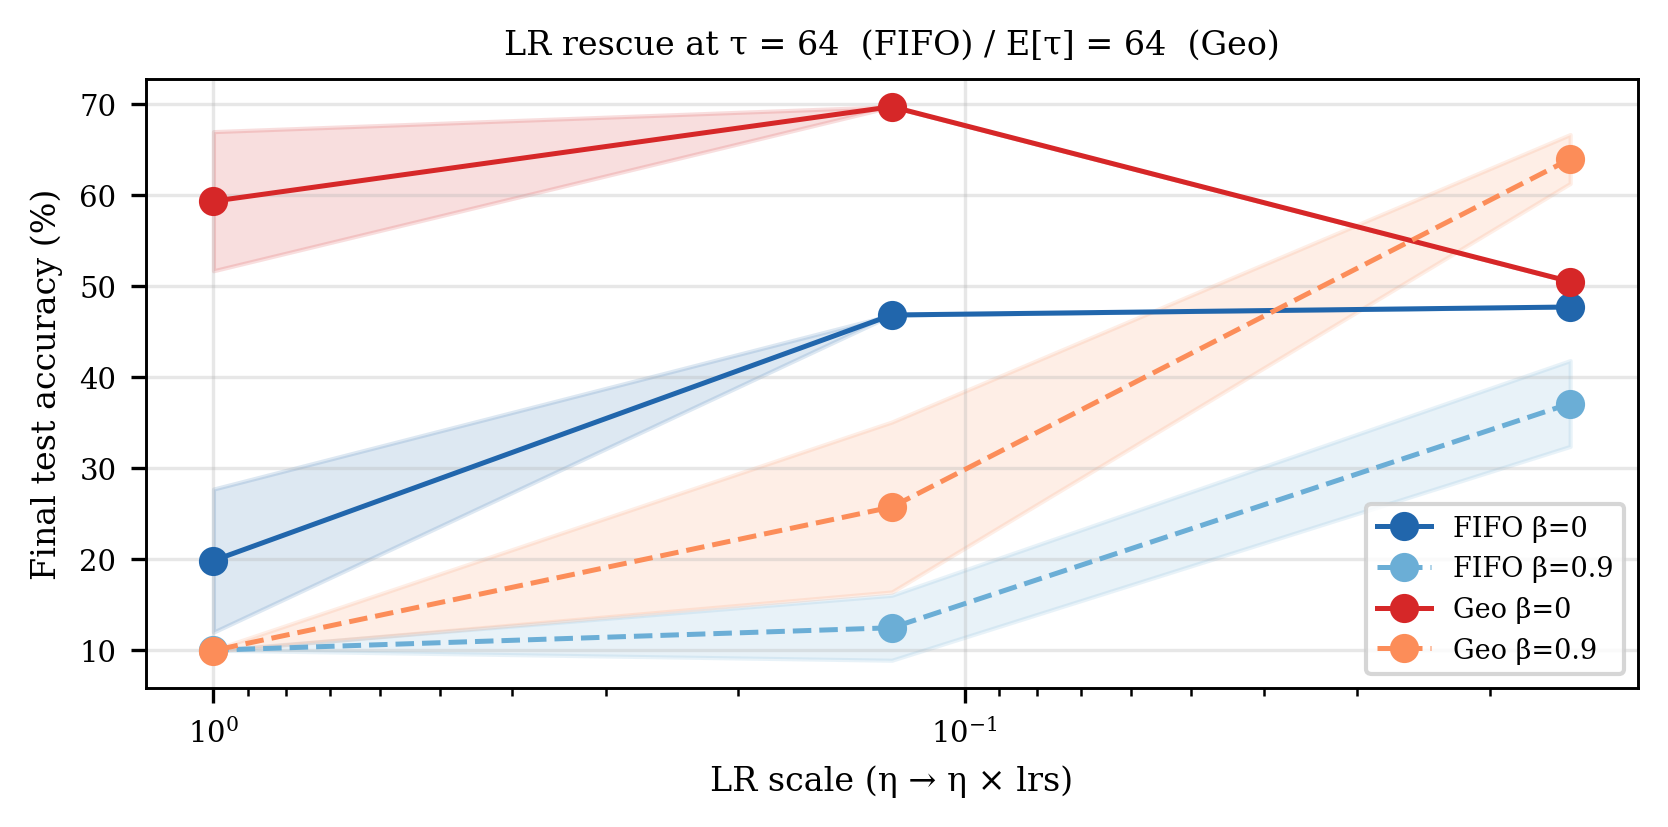
\includegraphics[width=\columnwidth]{plot_lrs_rescue}
  \caption{LR rescue at $\tau{=}64$ (FIFO) and $\mathrm{E}[\tau]{=}64$
           (geometric) for $\beta{\in}\{0,\,0.9\}$.
           For $\beta{=}0.9$, $\mathrm{lrs}{=}1/64$ is optimal (64.5\%
           geo vs.\ 31.3\% FIFO, $+33.2$\,pp).
           For $\beta{=}0$, $\mathrm{lrs}{=}1/\sqrt{64}$ is optimal;
           over-scaling to $1/64$ degrades accuracy.
           Shaded bands: $\pm1$\,s.d.\ over 3 seeds.}
  \label{fig:lrs-rescue}
\end{figure}

% =========================================================================
\subsection{Staleness and Regularization}
\label{sec:regularization}
% =========================================================================
In this section, we analyze how weight decay compares and interacts with
staleness.

\paragraph{Weight norm trajectories}
Figure~\ref{fig:weight-norm-traj-fifo} shows the weight $L_2$ norm
$\|w\|$ over 50 epochs for $\tau\in\{0,1,2,4,6,8,10\}$ at $\beta{=}0$ and no weight decay. The norm grows monotonically and the curves remain
nearly superimposed across all delays. Geometric delays give identical
results (Figure~\ref{fig:weight-norm-traj-geo}).


\paragraph{Weight decay and delay}
Figure~\ref{fig:tau_and_wd} reports final test accuracy as a function of
$\lambda$ for each $\tau$. Accuracy is flat and curves overlap for
$\lambda \leq 10^{-3}$, then collapse uniformly at $\lambda = 5\cdot 10^{-3}$
regardless of $\tau$.
\begin{figure}[tbp]
  \centering
  
\includegraphics[width=\columnwidth]{summary_l2_lambdasweep_fifo.png}
  \caption{Final top-1 test accuracy versus weight-decay coefficient
           $\lambda$, for $\tau\in\{0,1,2,4,6,8,10\}$
           (deterministic FIFO delay, $\beta{=}0$, no dropout, 50 epochs).
           Mean\,$\pm$\,1\,s.d.\ over 3 seeds.}
  \label{fig:tau_and_wd}
\end{figure} 

% =========================================================================
\section{Discussion}
% =========================================================================

Our results support a clear picture: momentum and gradient staleness
compound each other's harm, but the nature of this interaction depends
on the \emph{distribution} of delays, not just their average magnitude.
The most actionable finding is that LR correction ($\eta \to \eta/\tau$)
substantially rescues convergence at large delays --- and does so far more
effectively under stochastic (geometric) delay than under deterministic
FIFO delay: at $\mathrm{E}[\tau]{=}64$, $\mathrm{lrs}{=}1/64$ recovers
64.5\% (geometric) vs.\ 31.3\% (FIFO), a $+33.2$\,pp gap.

Under deterministic delay, the Liu et al.\ bound~\cite{liu2018momentum}
correctly predicts the instability regime and guides the adaptive schedule
design.
The finding that operating $\delta{=}0.3$ above the bound is empirically
safe suggests the bound is conservative, likely because it must hold for
arbitrary non-convex landscapes whereas CIFAR-10/ResNet-20 is comparatively
well-behaved after LR decay.

The Mitliagkas equivalence conjecture is not reproduced even under the
geometric delay distribution it was derived for.
The conjecture rests on a spectral equivalence derived for a linearised
(least-squares) model with stationary i.i.d.\ data: under those assumptions,
the update operator for $M$ geometric-delay workers maps exactly to an
explicit-momentum operator.
In a finite-epoch deep-learning setting, step-decay schedules violate this
stationarity by resetting the effective momentum horizon at each LR milestone.

\paragraph{Simulation scope and limitations.}
All findings are based on single-process gradient-buffer simulation.
Real async SGD introduces additional phenomena not modelled here: variable
worker speed, communication latency, memory consistency across processes,
and batch-norm statistics that diverge per worker.
Our results should therefore be interpreted as isolating the effect of
\emph{delay magnitude and distribution on the optimization dynamics}, not
as direct performance predictions for a production distributed system.

The convergence harm concentrates at the step-decay milestones, suggesting
that cosine or warmup-aware LR schedules --- which change the step size
gradually rather than in discrete drops --- would be more robust to gradient
staleness than the step-decay regime used here.

\paragraph{Regularization and staleness are uncorrelated}
While Deng et al.~\cite{deng2025generalizability} have studied how
gradient delay affects the generalization error of SGD, to our
knowledge, no prior work has examined how standard regularization
techniques such as weight decay interact with staleness. We do not
report dropout results here: dropout is not used in standard ResNet
architectures, as batch normalization already provides implicit
regularization, and the two mechanisms are known to interact
poorly~\cite{li2018understandingdisharmonydropoutbatch}.
Our results indicate that weight decay and staleness act along
independent axes. Figure~\ref{fig:weight-norm-traj-fifo} (and Figure ~\ref{fig:weight-norm-traj-geo}) show that
varying $\tau$ leaves the weight-norm trajectory essentially unchanged,
whereas Figure~\ref{fig:l2_wd_sweep} shows that $\lambda$ precisely
controls $\|w\|$ — small values let the norm grow freely, large values
actively shrink it. The two knobs therefore operate on different
quantities: $\lambda$ shapes the norm, $\tau$ does not. Consistently,
Figure~\ref{fig:tau_and_wd} shows that introducing delay on top of
weight decay neither amplifies nor mitigates the trends already
observed in the sequential ($\tau{=}0$) case: the $\lambda$-accuracy
curves for all $\tau$ overlap in the low-to-moderate regime and
collapse uniformly at $\lambda = 5\cdot 10^{-3}$. Weight decay tuned
for sequential training therefore transfers directly to the delayed
setting, with no need for $\tau$-aware adjustment.

\section{Summary}
% =========================================================================

Under zero-momentum FIFO training, delay degrades final accuracy
monotonically ($-29.5$\,pp from $\tau{=}0$ to $\tau{=}20$), with harm
concentrated at LR-decay milestones; scaling $\eta \to \eta/\tau$ is the
most effective remedy, recovering 64.5\% under geometric delay
vs.\ 31.3\% under FIFO at $\mathrm{E}[\tau]{=}64$ ($+33.2$\,pp, $\beta{=}0.9$).
The delay distribution matters as much as the magnitude: at
$\mathrm{E}[\tau]{=}20$, geometric delay retains 82.1\%
($+24.4$\,pp over FIFO) for $\beta{=}0$ but collapses faster than FIFO
for $\beta{=}0.9$, as rare extreme-lag events corrupt the momentum
accumulator.
$\beta{=}0.9$ collapses catastrophically under any FIFO delay
(10.6\% at $\tau{=}20$), consistent with the Liu et al.\
safe-momentum bound; an adaptive schedule tracking the bound recovers
up to $+5.9$\,pp, while the Mitliagkas implicit-momentum equivalence
does not hold even under the geometric regime it was derived for.
Weight decay and gradient staleness act on independent axes: varying $\tau$
leaves the weight-norm trajectory unchanged while $\lambda$ precisely
controls it; weight decay tuned for sequential training transfers directly
to the delayed setting with no need for $\tau$-aware adjustment.

\section*{Acknowledgements}
ResNet-20 implementation adapted from Idelbayev (public PyTorch
re-implementation of He et al.~\cite{he2016resnet}).
Compute provided by the EPFL IC RunAI cluster.

\newpage
\bibliographystyle{IEEEtran}
\bibliography{literature}

% =========================================================================
\newpage
\appendix
\section{Additional Figures}
% =========================================================================

\paragraph{Notation for Eq.~\eqref{eq:delayed-sgd}.}
$\theta_t \in \mathbb{R}^d$ is the parameter vector; $\eta_t > 0$ the
learning rate; $g(\theta) = \nabla f(\theta)$ the gradient of the
objective; $\tau_t \in \mathbb{N}$ the staleness (number of updates
elapsed between gradient computation and application).

\begin{figure}[htbp]
  \centering
  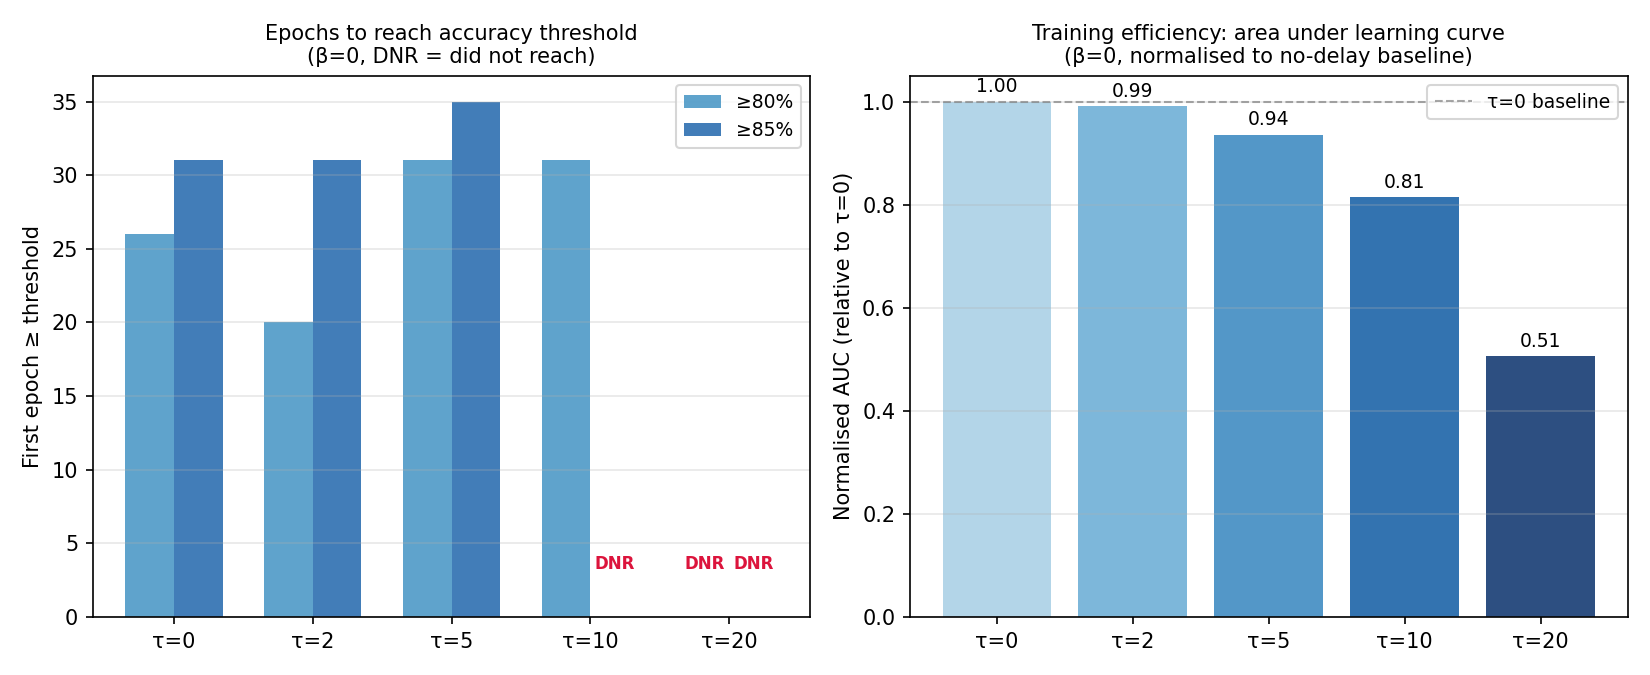
\includegraphics[width=\columnwidth]{plot_Q1_convergence_metrics}
  \caption{Left: first epoch reaching 80\%/85\% test accuracy under
           $\beta{=}0$ (DNR~= did not reach within 50 epochs).
           Right: normalised AUC of the learning curve relative to the
           $\tau{=}0$ baseline; $\tau{=}20$ retains only half the
           training efficiency.}
  \label{fig:q1-metrics}
\end{figure}

\begin{figure}[htbp]
  \centering
  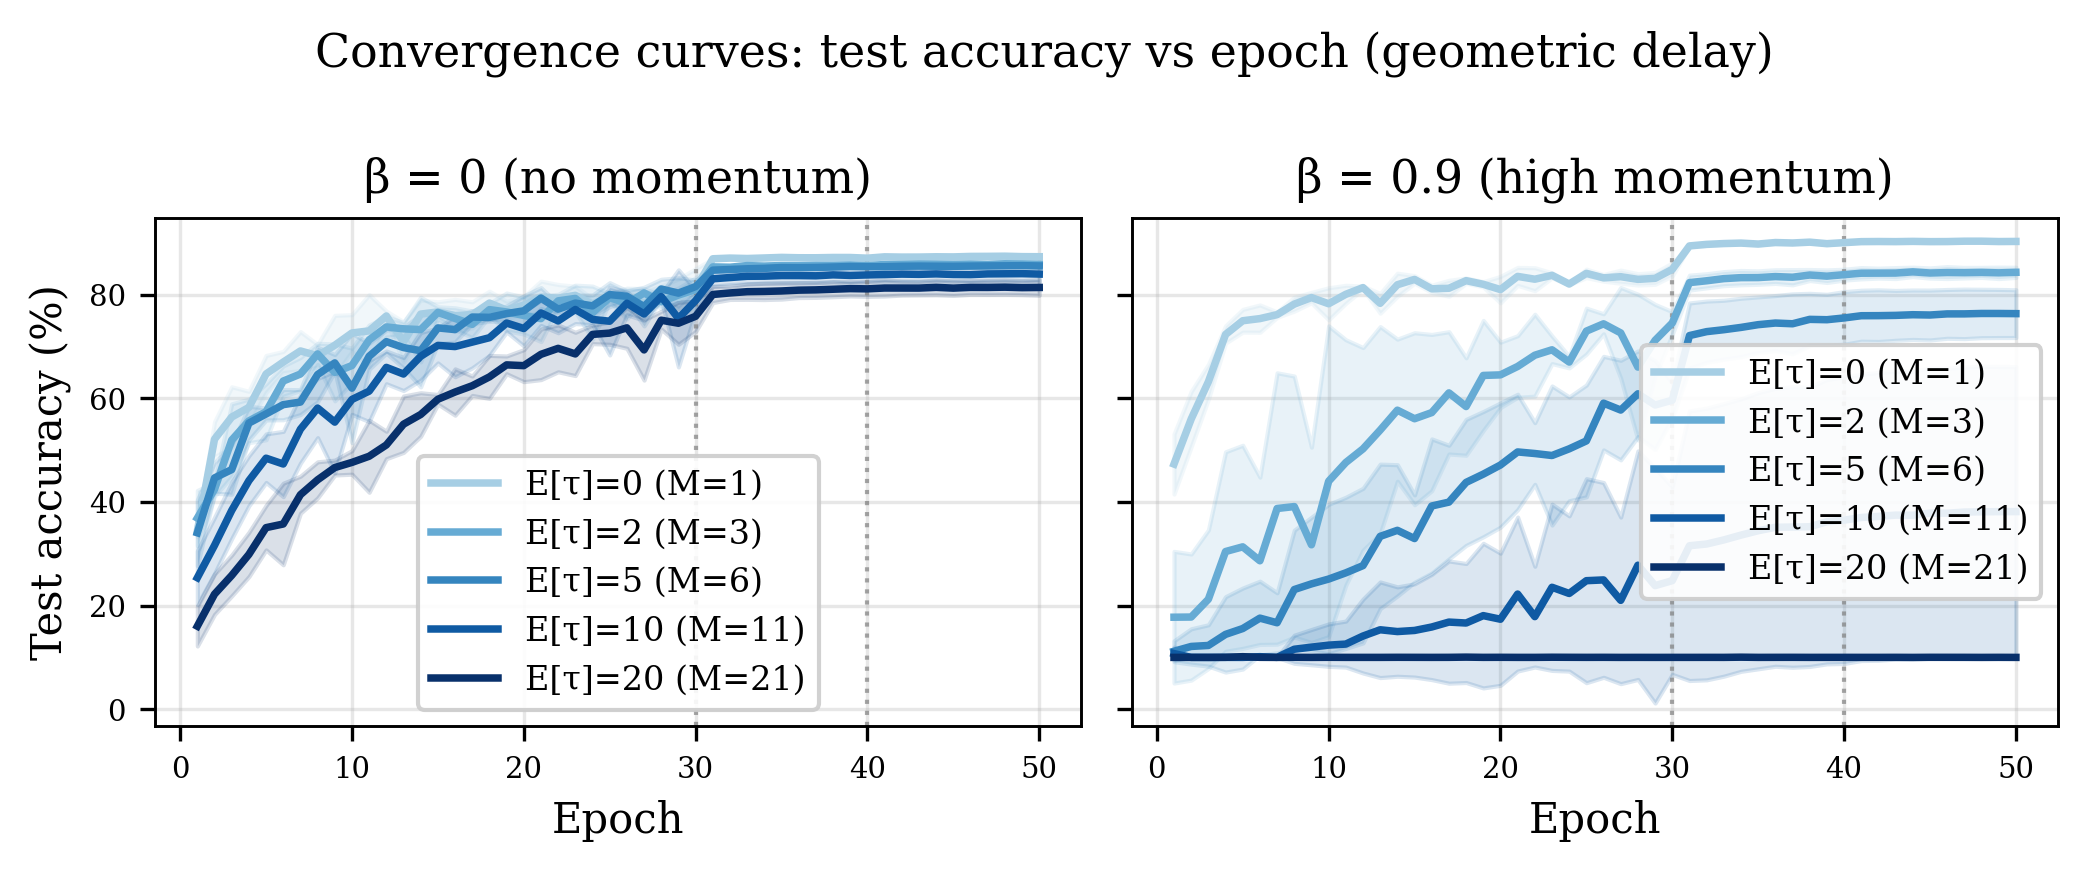
\includegraphics[width=\columnwidth]{plot_Q1_geo_convergence_curves}
  \caption{Test accuracy vs.\ epoch for $\beta{=}0$ (left) and $\beta{=}0.9$
           (right) across $\mathrm{E}[\tau] \in \{0,2,5,10,20\}$ (geometric
           delay). Degradation is milder for $\beta{=}0$ but more severe for
           $\beta{=}0.9$ compared to deterministic delay.}
  \label{fig:q1-geo-curves}
\end{figure}

\begin{figure}[htbp]
  \centering
  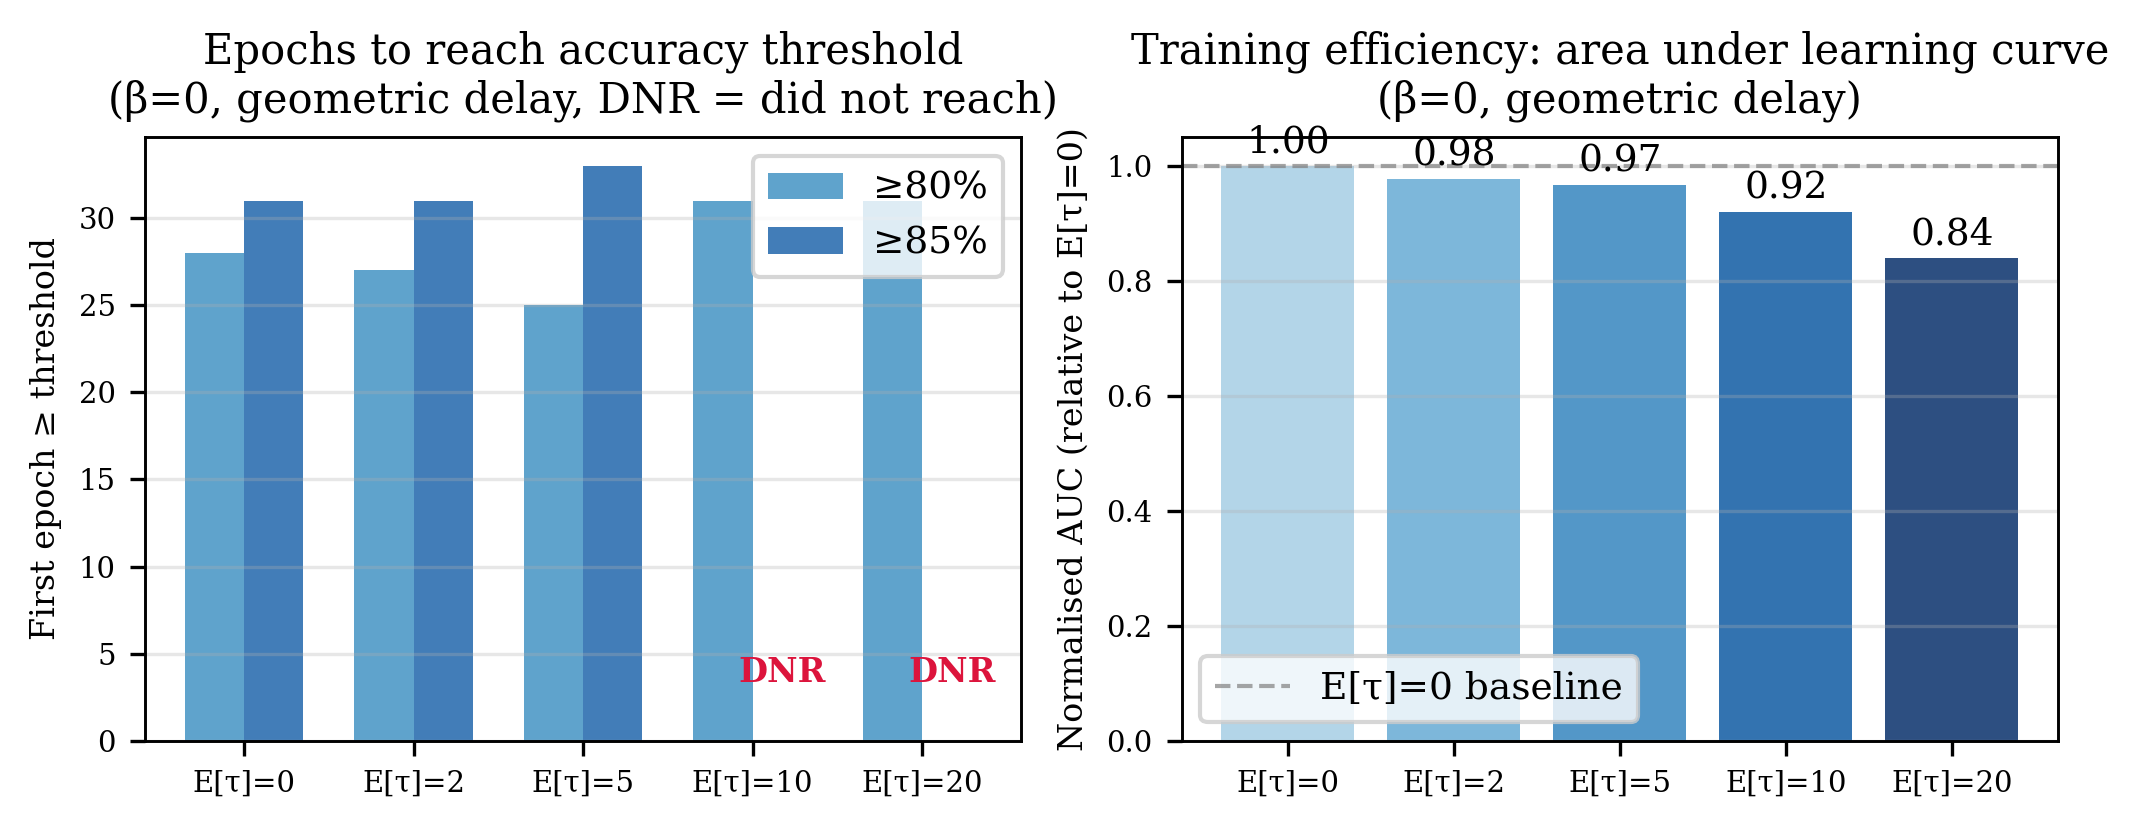
\includegraphics[width=\columnwidth]{plot_Q1_geo_convergence_metrics}
  \caption{Epochs-to-threshold and normalised AUC under geometric delay
           ($\beta{=}0$). Geometric delay degrades AUC less steeply than
           deterministic delay (Fig.~\ref{fig:q1-metrics}).}
  \label{fig:q1-geo-metrics}
\end{figure}

\begin{figure}[htbp]
  \centering
  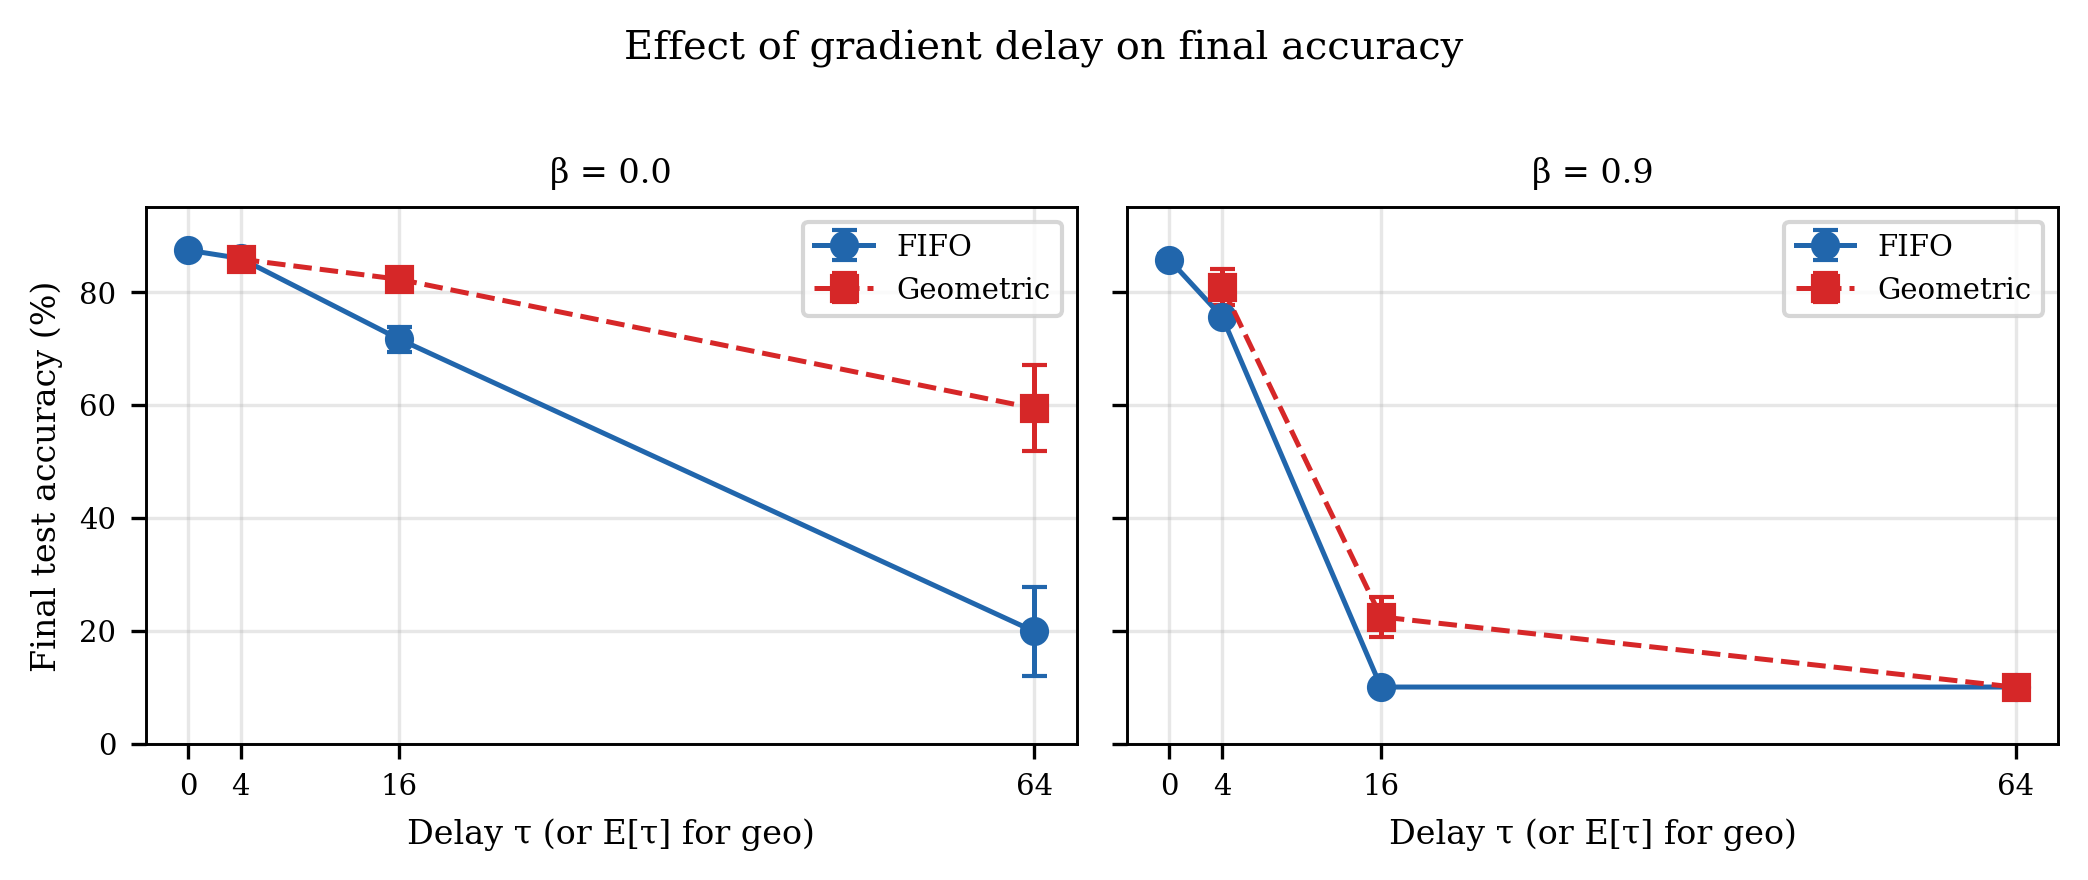
\includegraphics[width=\columnwidth]{plot_step5_grid}
  \caption{Final test accuracy vs.\ gradient staleness for $\beta{=}0$
           (left) and $\beta{=}0.9$ (right) under FIFO and geometric delay
           ($\mathrm{lrs}{=}1$, mean $\pm$ std, 3 seeds).
           For $\beta{=}0$, geometric delay retains 60\% at $\tau{=}64$
           vs.\ 20\% under FIFO; for $\beta{=}0.9$, both regimes collapse
           at high delay.}
  \label{fig:step5-grid}
\end{figure}

\begin{figure}[htbp]
  \centering
  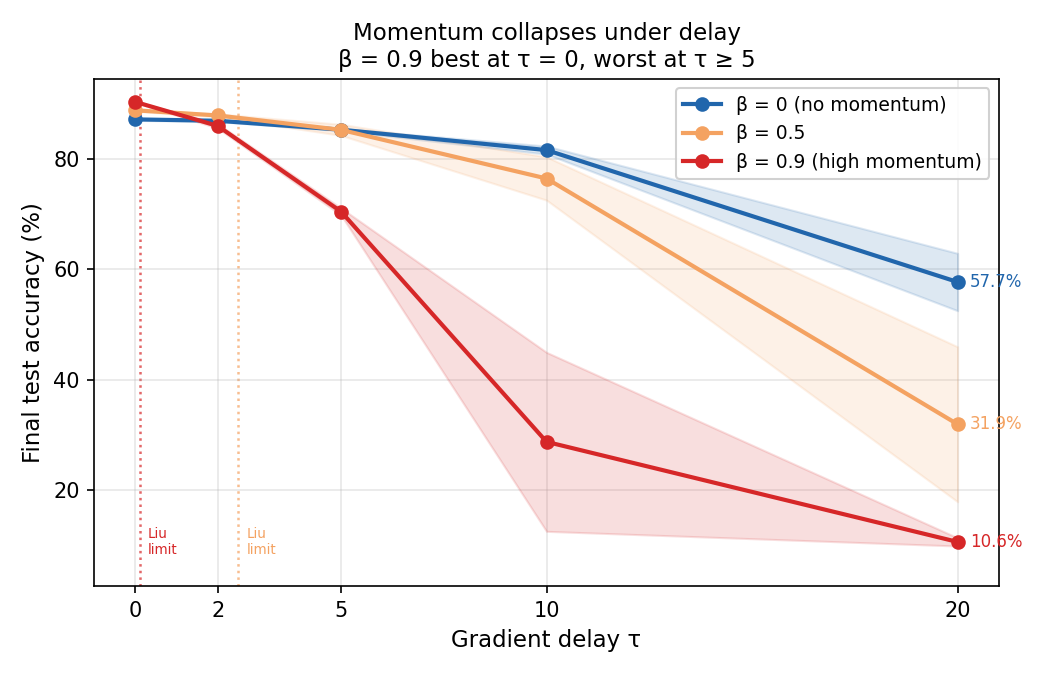
\includegraphics[width=\columnwidth]{plot_C_momentum_benefit}
  \caption{Final test accuracy vs.\ delay $\tau$ for three fixed momentum
           values (deterministic delay). $\beta{=}0.9$ is best at $\tau{=}0$
           but collapses under any delay; $\beta{=}0$ is most robust.
           Mean $\pm$ std, 3 seeds.}
  \label{fig:momentum-collapse}
\end{figure}

\begin{figure}[htbp]
  \centering
  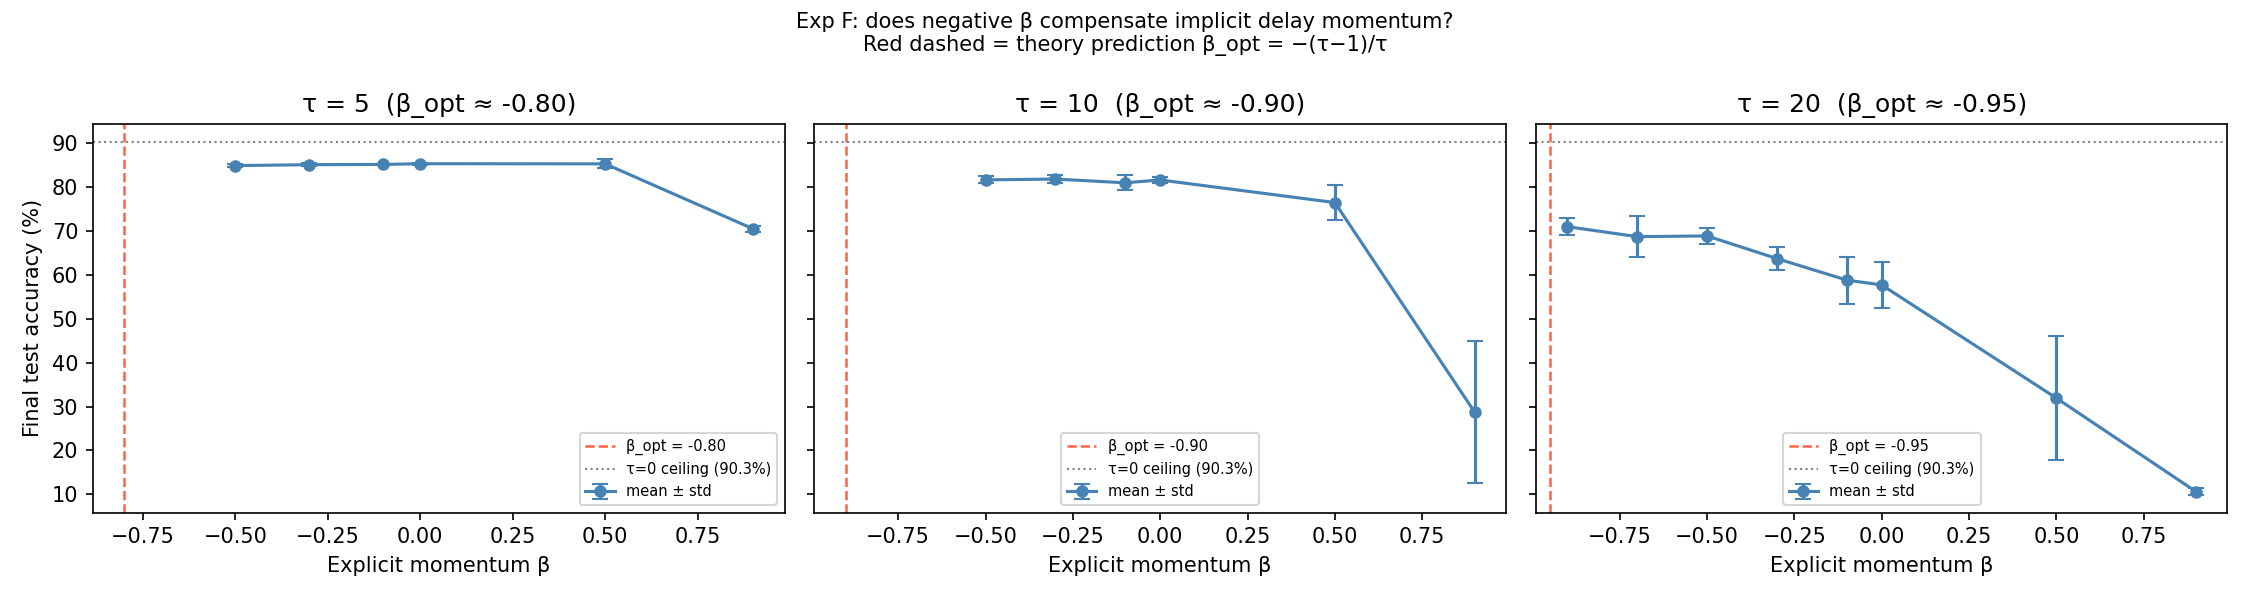
\includegraphics[width=\columnwidth]{plot_K_negative_momentum}
  \caption{Exp~F: negative explicit momentum sweep at
           $\tau \in \{5,10,20\}$ (deterministic delay).
           Negative $\beta$ improves over $\beta{=}0$ at $\tau{=}20$
           (peak gain 13.3\,pp at $\beta{=}{-}0.9$) but underperforms
           at $\tau{=}5$.}
  \label{fig:neg-momentum}
\end{figure}

\begin{figure}[htbp]
  \centering
  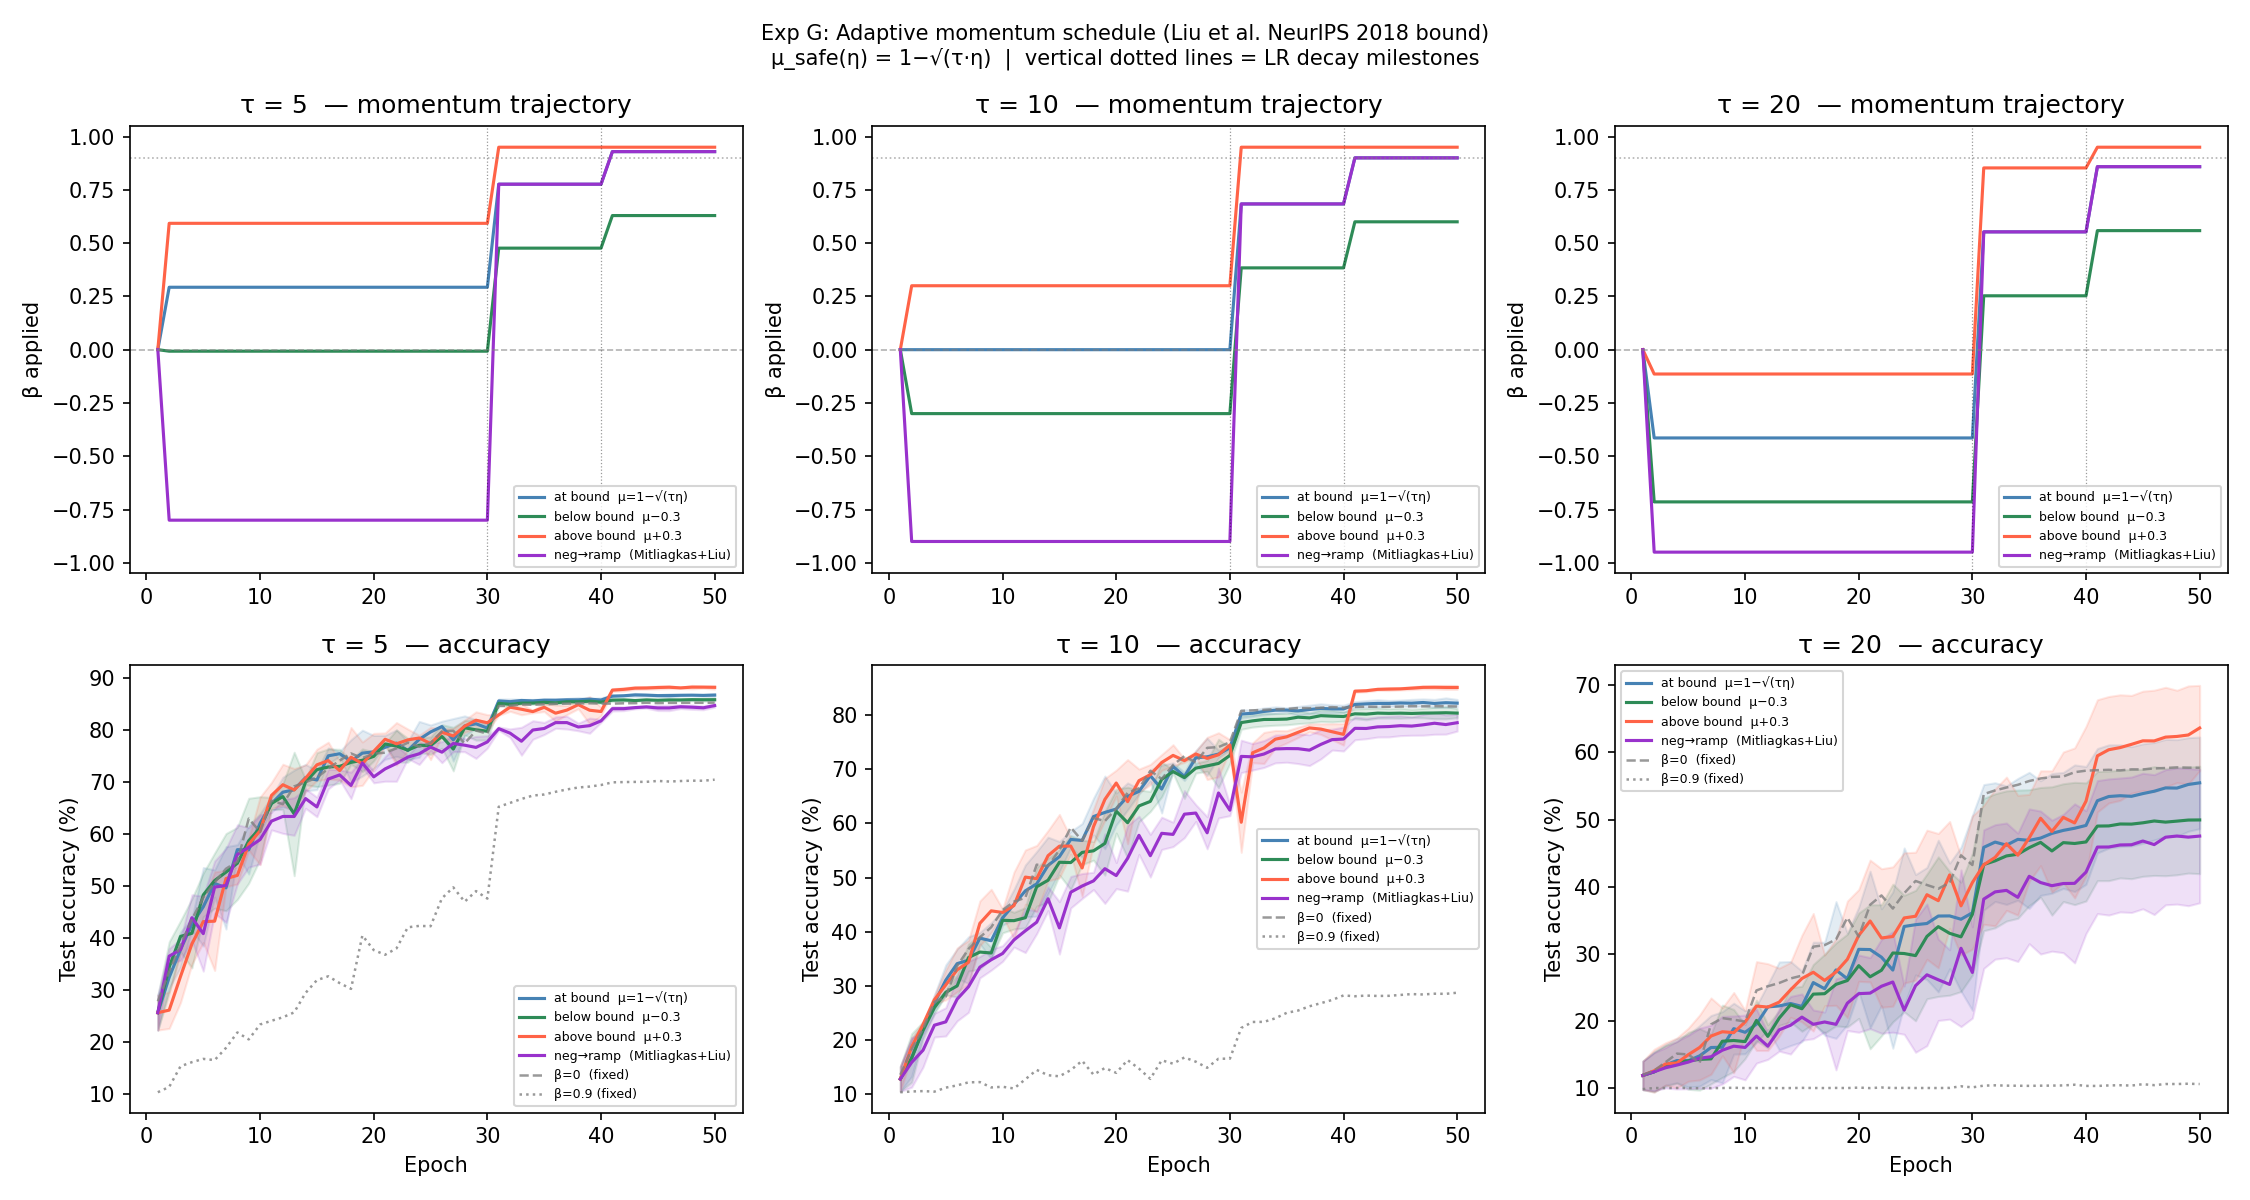
\includegraphics[width=\columnwidth]{plot_L1_adaptive_curves}
  \caption{Exp~G: per-epoch convergence curves for four adaptive
           schedules at each $\tau$ (deterministic delay).
           \texttt{above\_bound} converges faster and to a higher
           final accuracy at all delays.}
  \label{fig:adaptive-curves}
\end{figure}

\begin{figure}[htbp]
  \centering
  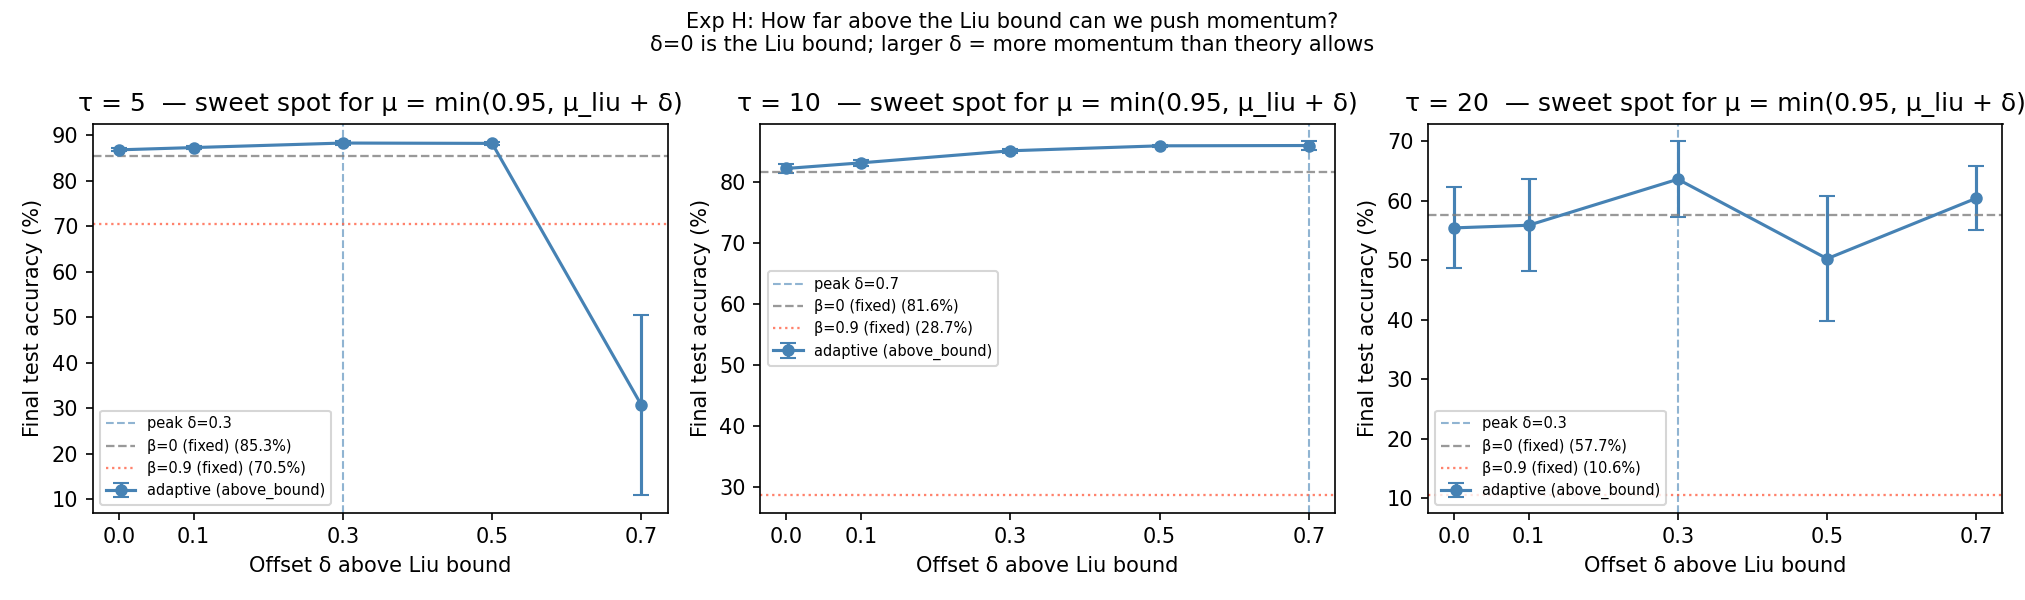
\includegraphics[width=\columnwidth]{plot_M_above_bound_sweep}
  \caption{Exp~H: sweet-spot sweep for the offset $\delta$ above the Liu
           bound ($\mu = \min(0.95,\,\mu_\mathrm{safe} + \delta)$) at
           $\tau \in \{5, 10, 20\}$.
           $\delta{=}0.3$ is consistently best or tied-best across all
           delays; larger offsets ($\delta \geq 0.5$) degrade at high~$\tau$.}
  \label{fig:above-bound-sweep}
\end{figure}

\begin{figure}[htbp]
  \centering
  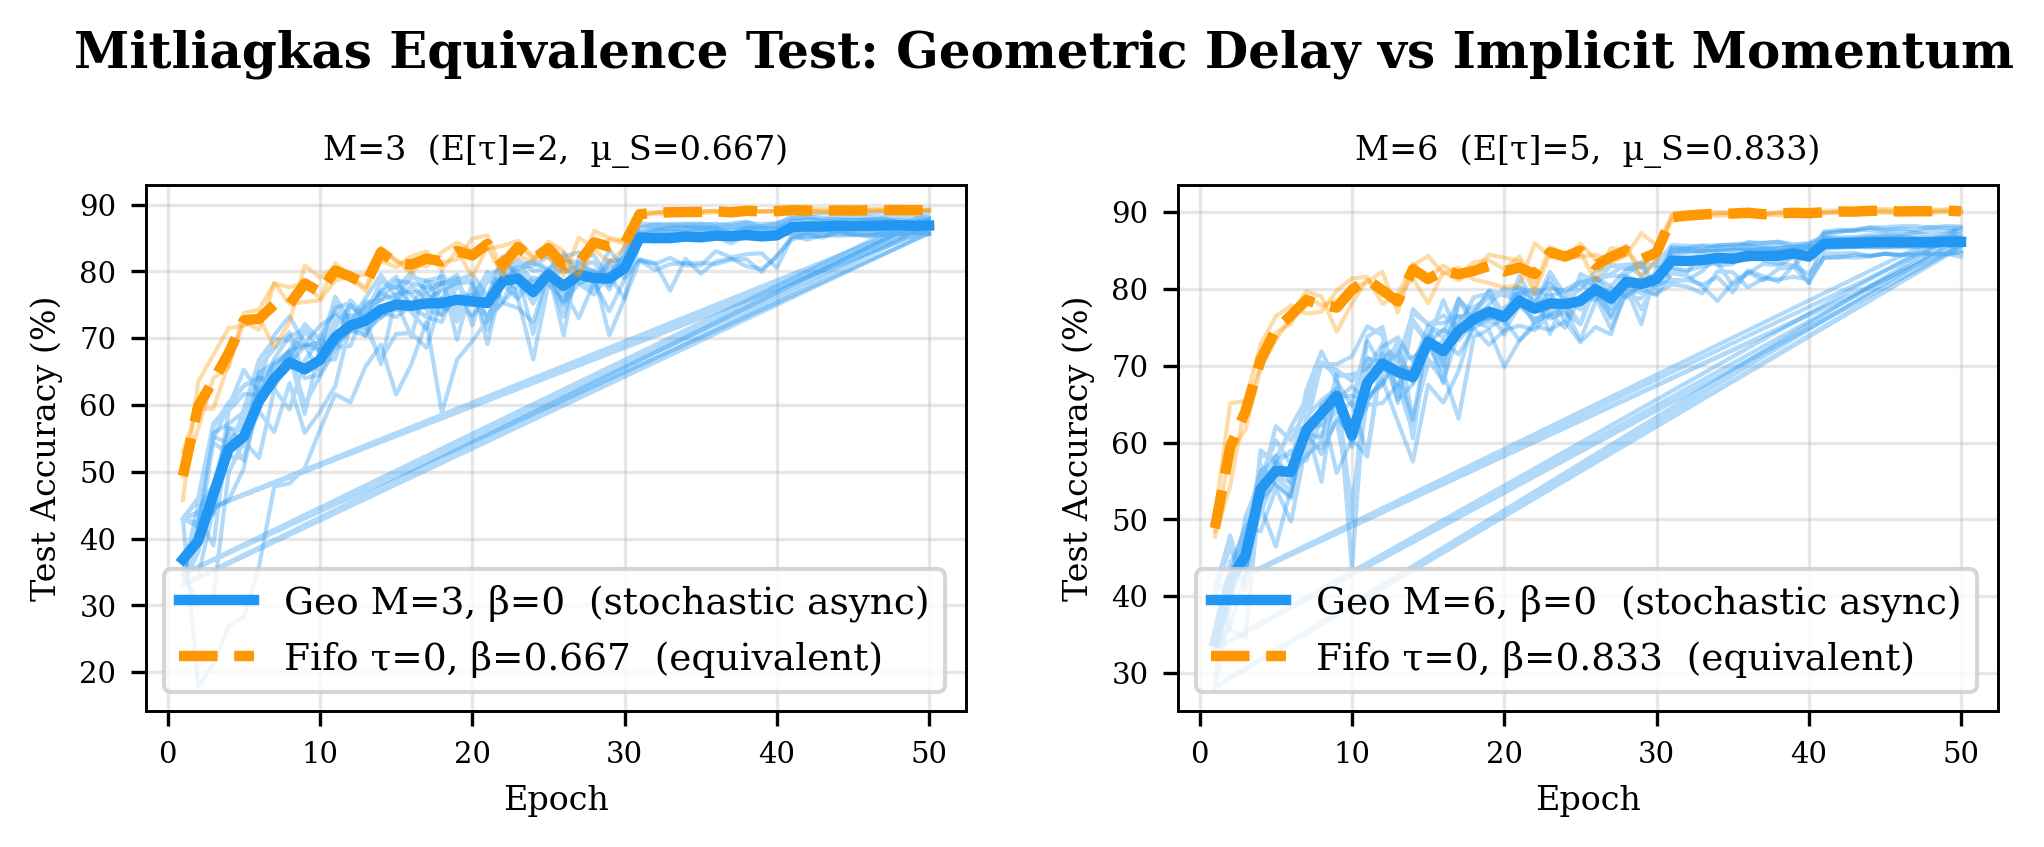
\includegraphics[width=\columnwidth]{plot_geo_equivalence}
  \caption{Mitliagkas equivalence test under geometric delay.
           Geo $M{=}3$/$M{=}6$ with $\beta{=}0$ (blue) vs.\
           deterministic $\tau{=}0$ with $\beta{=}\mu_S$ (orange).
           The equivalence does not hold empirically even under the
           geometric distributional assumption of the original proof.}
  \label{fig:geo-equivalence}
\end{figure}

\begin{figure}[htbp]
  \centering
  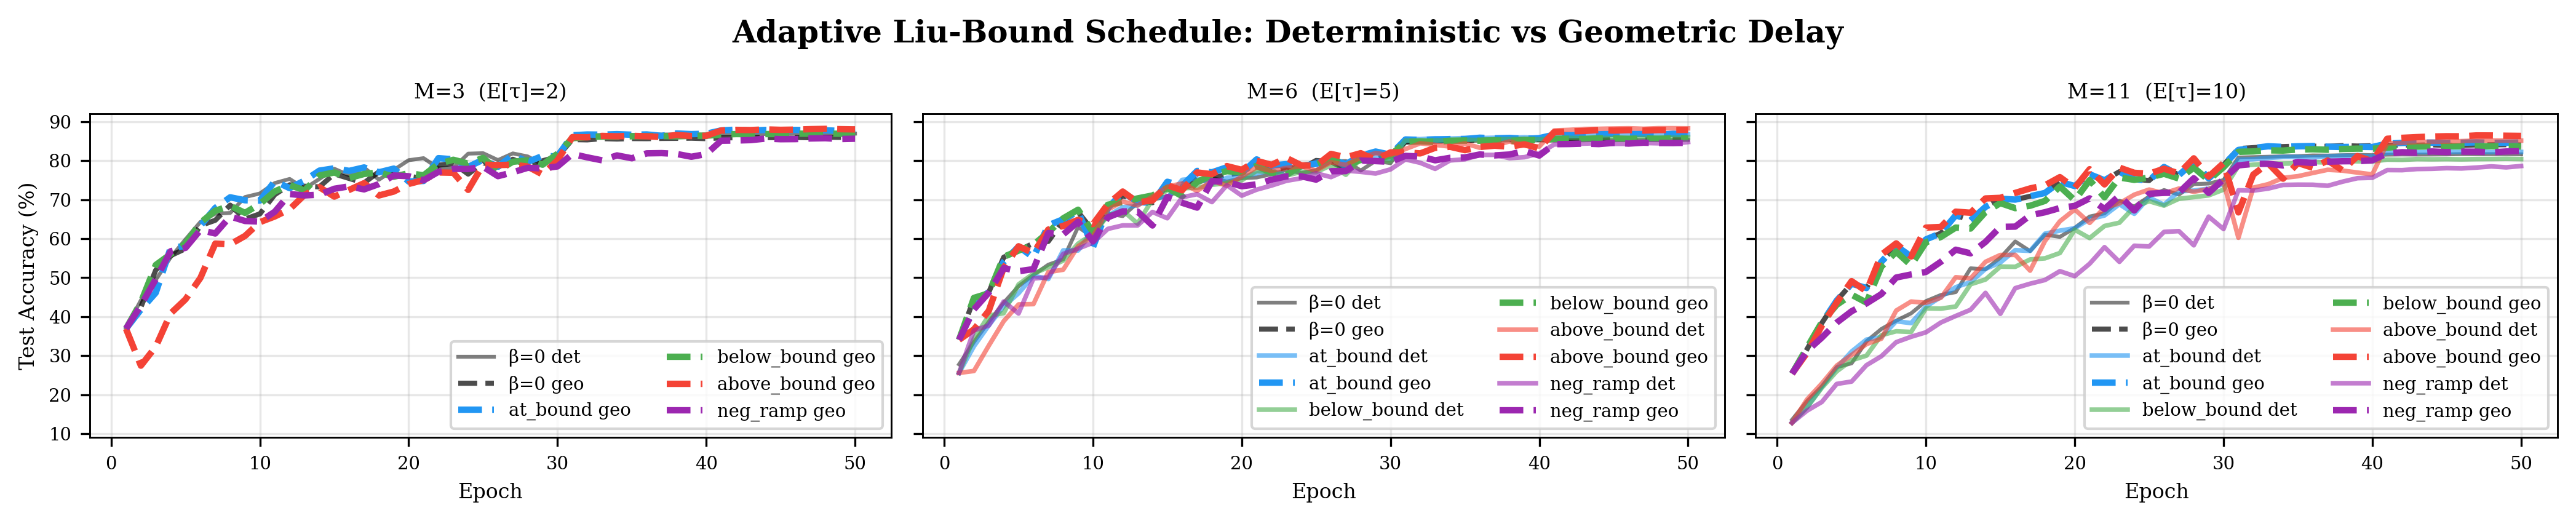
\includegraphics[width=\columnwidth]{plot_geo_adaptive}
  \caption{Exp~G under geometric delay: adaptive Liu-bound schedule
           (dashed) vs.\ deterministic delay (solid) at matched
           $\mathrm{E}[\tau]$. Black lines show the $\beta{=}0$
           reference. \texttt{above\_bound} remains the best schedule
           under geometric delay, but with larger variance.}
  \label{fig:geo-adaptive}
\end{figure}



\begin{figure}[htbp]
  \centering
  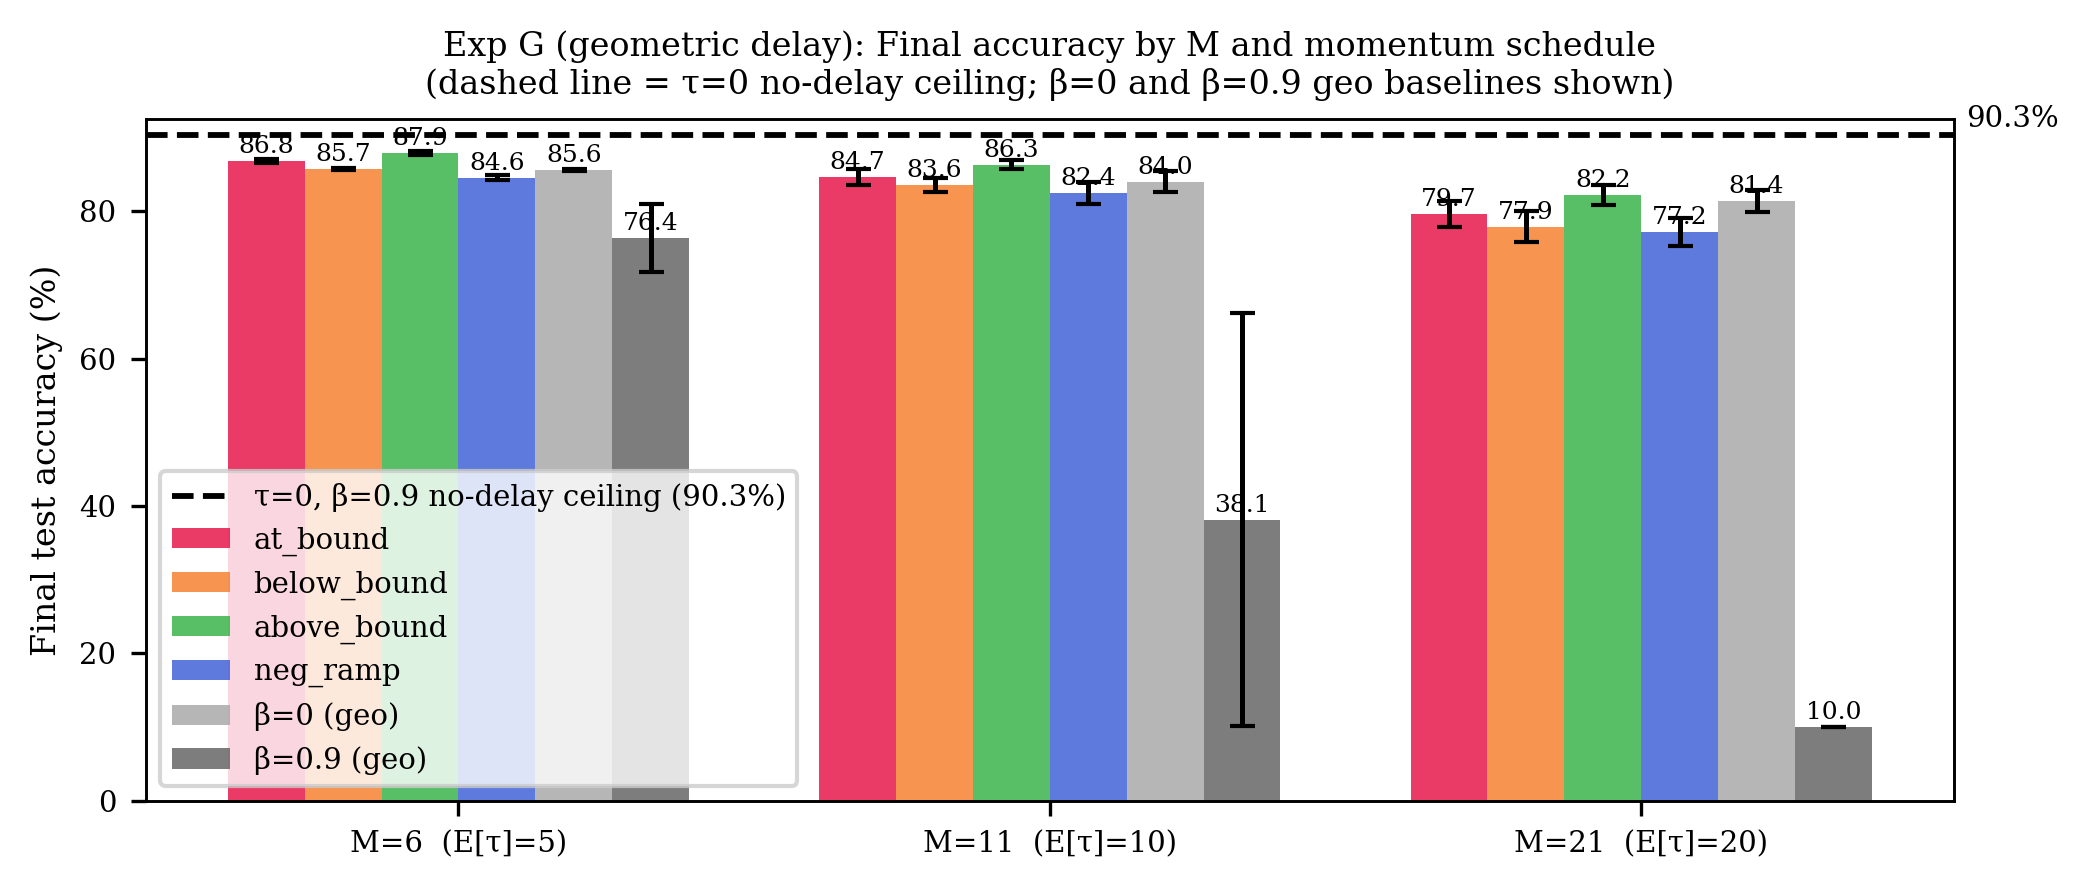
\includegraphics[width=\columnwidth]{plot_geo_L2_adaptive_summary}
  \caption{Exp~G (geometric delay): final test accuracy by $M$ and
           momentum schedule (cf.\ Fig.~\ref{fig:adaptive-summary} for
           the deterministic counterpart). Adaptive schedules consistently
           outperform the $\beta{=}0.9$ geometric baseline (which
           collapses to 10.0\% at $M{=}21$) and approach the $\beta{=}0$
           ceiling; \texttt{above\_bound} is best at all three $M$ values.}
  \label{fig:geo-adaptive-summary}
\end{figure}

\begin{figure}[htbp]
  \centering
  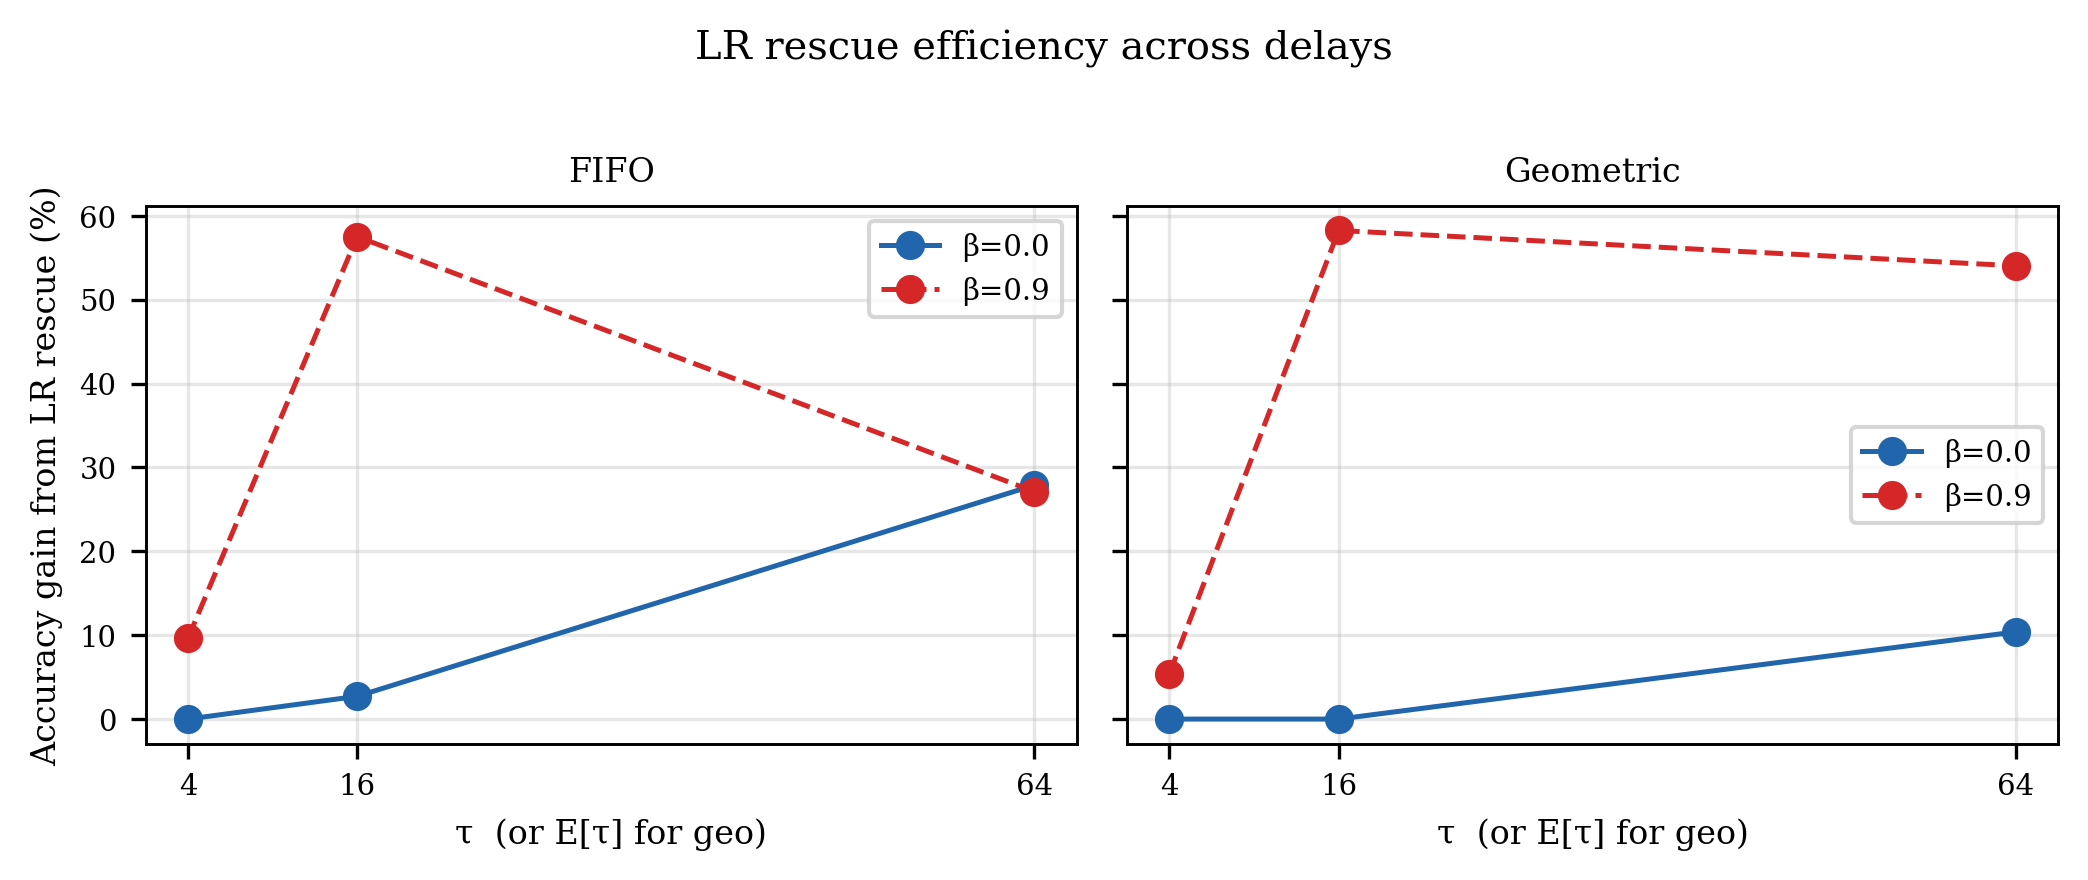
\includegraphics[width=\columnwidth]{plot_lrs_rescue_sweep}
  \caption{LR rescue efficiency across $\tau \in \{4,16,64\}$ for FIFO
           (left) and geometric (right). $y$-axis: accuracy gain from
           best-lrs over lrs$=1$ baseline. For $\beta{=}0.9$, gains are
           large at moderate delays ($\tau{=}16$) and remain high under
           geometric delay at $\tau{=}64$; for $\beta{=}0$, gains are
           modest and grow slowly with $\tau$.}
  \label{fig:lrs-rescue-sweep}
\end{figure}

\begin{figure}[htbp]
  \centering
  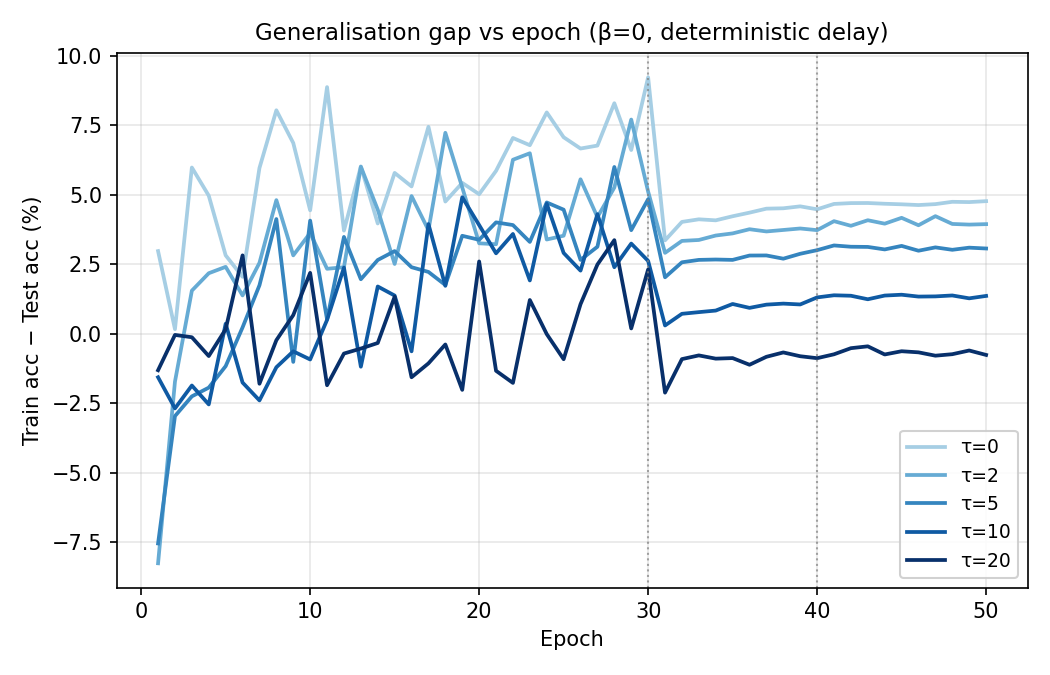
\includegraphics[width=\columnwidth]{plot_Q1_train_test_gap}
  \caption{Train-test accuracy gap (train\,$-$\,test) vs.\ epoch for
           $\beta{=}0$ across $\tau \in \{0,2,5,10,20\}$ (deterministic
           delay). The gap narrows as $\tau$ increases, consistent with
           Deng et al.~\cite{deng2025generalizability}: gradient delay
           improves algorithmic stability, reducing generalisation error.}
  \label{fig:q1-gap}
\end{figure}

\begin{figure}[htbp]
  \centering
  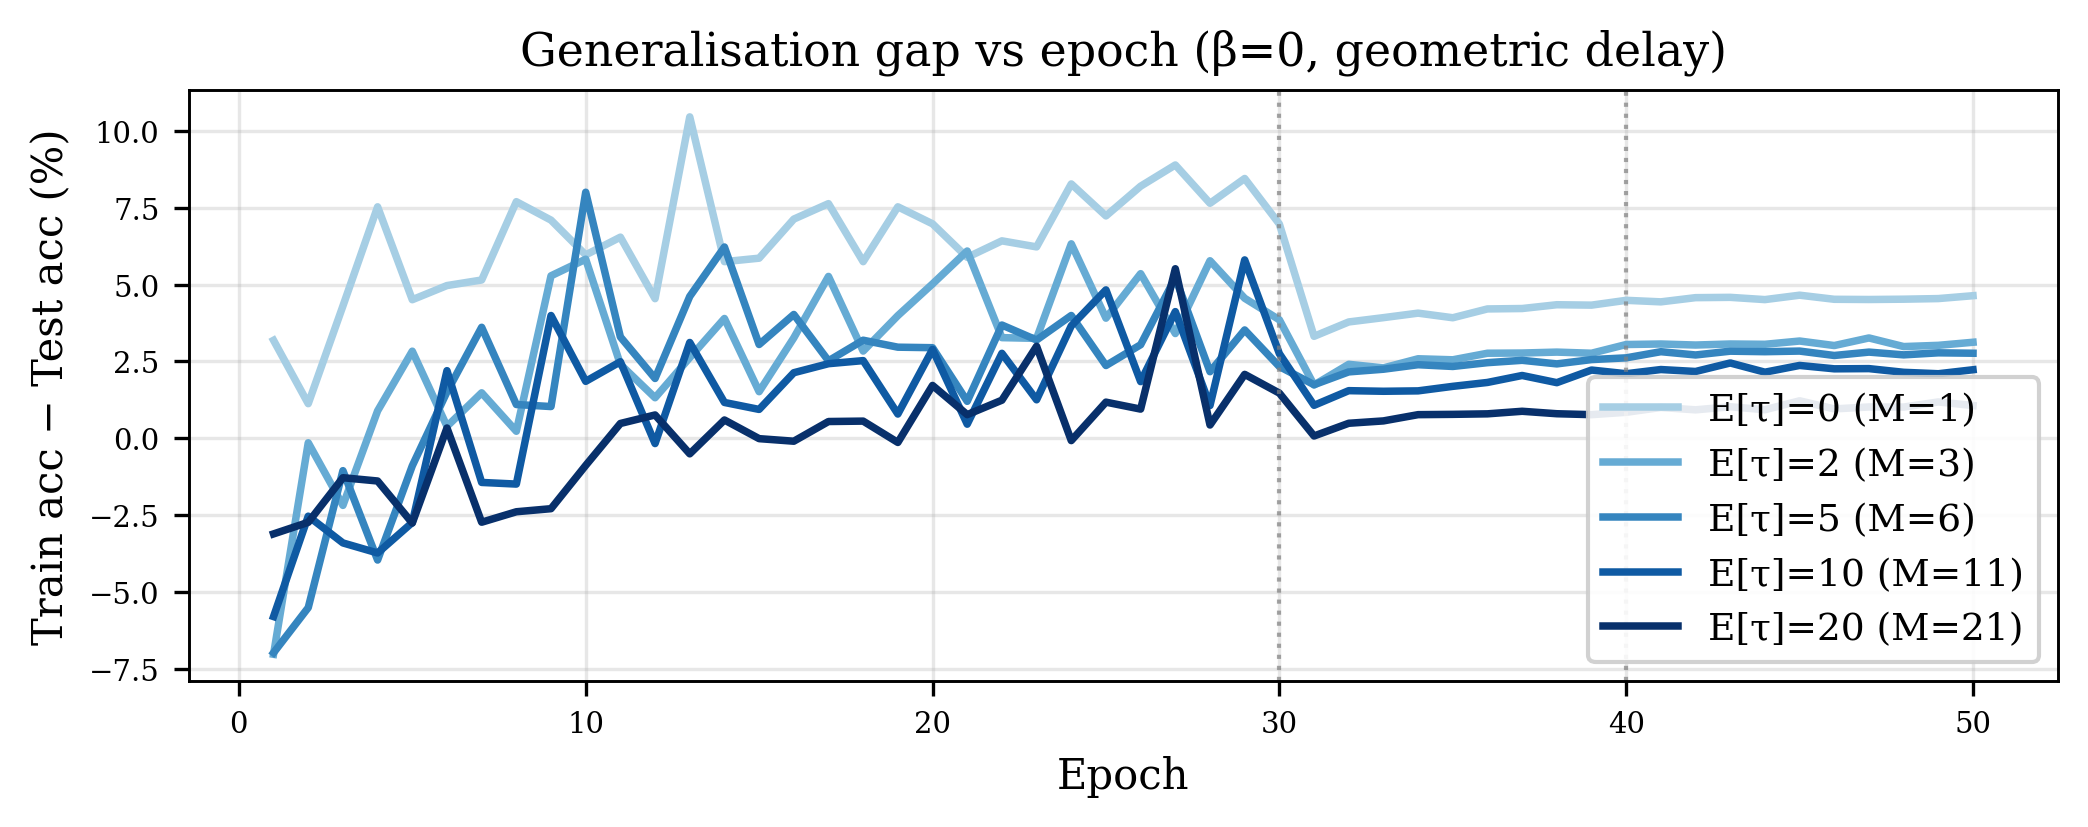
\includegraphics[width=\columnwidth]{plot_Q1_geo_train_test_gap}
  \caption{Train-test accuracy gap vs.\ epoch for $\beta{=}0$ across
           $\mathrm{E}[\tau] \in \{0,2,5,10,20\}$ (geometric delay).
           Same narrowing pattern as the deterministic case
           (Fig.~\ref{fig:q1-gap}).}
  \label{fig:q1-geo-gap}
\end{figure}


%---------------------------------------
% Extension Figures For Results – Aleks
%---------------------------------------
\begin{figure}[tbp]
  \centering
  
\includegraphics[width=\columnwidth]{weight_norm_beta_tausweep_m_0.0_geometric.png}
  \caption{Weight L2 norm $\|w\|$ over training for
           $M\in\{1,2,3,5,7,9,11\}$ (geometric delay, $\beta{=}0$, no dropout,
           no weight decay). All curves grow monotonically and remain
           nearly superimposed across all 50 epochs;
           mean\,$\pm$\,1\,s.d.\ over 3 seeds.}
  \label{fig:weight-norm-traj-geo}
\end{figure}



\begin{figure}[tbp]
  \centering
  
\includegraphics[width=\columnwidth]{weight_norm_beta_tausweep_m_0.0_fifo.png}
  \caption{Weight $L_2$ norm $\|w\|$ over training for
           $\tau\in\{0,1,2,4,6,8,10\}$ (deterministic delay, $\beta{=}0$,
           no dropout, no weight decay). Mean\,$\pm$\,1\,s.d.\ over 3 seeds.}
  \label{fig:weight-norm-traj-fifo}
\end{figure}


\begin{figure}[tbp]
  \centering
  
\includegraphics[width=\columnwidth]{weight_norm_l2sweep_m_0.0.png}
  \caption{Weight L2 norm $\|w\|$ over seq training for
           $\lambda \in\{0, 1e-5, 5e-5, 1e-4, 5e-4, 1e-3, 5e-3\}$ ($\beta{=}0$ and no dropout).
           mean\,$\pm$\,1\,s.d.\ over 3 seeds.}
  \label{fig:l2_wd_sweep}
\end{figure} 

% \begin{figure}[tbp]
%   \centering
%   \includegraphics[width=\columnwidth]{l2_sweep.png}
%   \caption{Write it out}
%   \label{fig:tau_and_wd}
% \end{figure} 
%---------------------------------------

\end{document}
